\documentclass[11pt]{article}
\usepackage[dvipsnames]{xcolor}
\usepackage{times}
\usepackage{amsmath,amsthm,amssymb,setspace,enumitem,epsfig,titlesec,verbatim,array,eurosym,multirow}
\usepackage[sort&compress,numbers]{natbib}
\usepackage[footnotesize,bf]{caption}
\usepackage[margin=2.5cm, includefoot, footskip=30pt]{geometry}
\usepackage{standalone}
\usepackage{tikz}
\usepackage{subcaption}
\usepackage{hyperref}
\usepackage{tabularx}
\usepackage{booktabs}
\usepackage{blkarray}
\usepackage[ruled,vlined]{algorithm2e}
\smallskip % Erlaubt kleine Abstaende zwischen Paragraphen, falls es dem Seitenlayout hilft
\renewcommand{\baselinestretch}{1.3}
\newcommand{\R}{\mathbb{R}}

\usetikzlibrary{decorations.pathreplacing, backgrounds, fit, calc, matrix, positioning}

\definecolor{darkblue}{rgb}{0,0,.8}
\definecolor{darkgreen}{rgb}{0,0.5,0.1}
\definecolor{lightapricot}{rgb}{0.99, 0.84, 0.69}
\newcommand{\matlabfunc}[1]{\textcolor{darkblue}{#1}}
\newcommand{\matlabcomment}[1]{\textcolor{darkgreen}{#1}}
\newcommand{\christian}[1]{\textcolor{blue}{\textbf{CH}: #1}}
\newcommand{\alex}[1]{\textcolor{red}{\textbf{AL}: #1}}

\def\alld{\texttt{ALLD}}
\def\tft{\texttt{TFT}}
\def\gtft{\texttt{GTFT}}
\def\rolemodel{\text{R}}
\def\learner{\text{L}}
\def\resident{\texttt{R}}
\def\mutant{\texttt{M}}
\def\strategy{\texttt{$\sigma$}}
\def\esm{electronic supplementary material}

\definecolor{expectedcolor}{rgb}{0.1791464821222607, 0.49287197231833907, 0.7354248366013072}
\definecolor{oneone}{rgb}{0.8503344867358708, 0.14686658977316416, 0.13633217993079583}
\definecolor{onetwo}{rgb}{0.18246828143021915, 0.5933256439830834, 0.3067589388696655}
\definecolor{twoone}{rgb}{0.4488427527873895, 0.3839600153787005, 0.6738792772010764}
\definecolor{twotwo}{rgb}{0.8871510957324106, 0.3320876585928489, 0.03104959630911188}


%% Adding shortcut commands to refer to our figures %%
\newcommand{\FigEvoProc}{{\bf Fig.~1}} \newcommand{\FigInvAnalysis}{{\bfFig.~2}} \newcommand{\FigResultsOverPara}{{\bf Fig.~3}}


\titleformat{\section}{\sffamily \fontsize{12}{14}\bfseries}{\thesection}{1em}{}
\titleformat{\subsection}{\sffamily
\fontsize{11.5}{11.5}\bfseries}{\thesubsection}{1em}{}

\usepackage{tikz}
\usetikzlibrary{arrows}

\tikzset{treenode/.style = {align=center, inner sep=0pt, text centered,
  font=\sffamily}, arn_n/.style = {treenode, circle, white,
  font=\sffamily\bfseries, draw=black, inner sep=-6pt, fill=black, text
  width=1.5em},% arbre rouge noir, noeud noir
  arn_r/.style = {treenode, circle, red, text width=1.5em, very thick, inner
    sep=4pt},% arbre rouge noir, noeud rouge
  arn_x/.style = {treenode, rectangle, draw=black, minimum width=0.5em, minimum
    height=0.5em}% arbre rouge noir, nil
}

\newtheoremstyle{plainCl1}% name
{9pt}%      Space above, empty = 'usual value'
{9pt}%      Space below
{\it}% 	   Body font
{}%         Indent amount (empty = no indent, \parindent = para indent)
{\bfseries}% Thm head font
{.}%        Punctuation after thm head
{0.2cm}% Space after thm head: \newline = linebreak
{}%         Thm head spec

\newtheoremstyle{plainCl2}% name
{9pt}%      Space above, empty = 'usual value'
{9pt}%      Space below
{\it}% 	   Body font
{}%         Indent amount (empty = no indent, \parindent = para indent)
{\bfseries}% Thm head font
{$'$.}%        Punctuation after thm head
{0.2cm}% Space after thm head: \newline = linebreak
{}%         Thm head spec

\newcommand{\splitatcommas}[1]{%
  \begingroup
  \begingroup\lccode`~=`, \lowercase{\endgroup \edef~{\mathchar\the\mathcode`,
    \penalty0 \noexpand\hspace{0pt plus 1em}}%
  }\mathcode`,="8000 #1%
  \endgroup
}

\theoremstyle{plainCl1}
\newtheorem{Claim}{Claim}
\newtheorem{Thm}{Theorem}
\newtheorem{Prop}{Proposition}
\newtheorem*{Lem}{Lemma}
\newtheorem{Cor}{Corollary}
\newtheorem*{Def}{Definition}

\theoremstyle{plainCl2}
\newtheorem{Claim2}{Claim}

\title{{ \sffamily \LARGE Electronic supplementary material}\\{\bf \sffamily \LARGE Evolution of reciprocity with limited payoff memory}}
\date{}
\author{Nikoleta E. Glynatsi, Alex McAvoy,  Christian Hilbe}

\begin{document}
\maketitle


%% BRIEF INTRO %% 

\noindent
This document provides further details on our methods and derivations, and it contains additional simulation results. 
Section~\ref{section:model} summarizes the model. 
In particular, we provide further details on our implementation of the evolutionary dynamics, and our use of the rare-mutations limit. 
In Section~\ref{section:analyticalresults} we derive analytical results for the various settings we consider.
These settings differ in what kind of payoff information individuals take into account when updating their strategies. 
In the perfect memory setting, individuals take into account all their interactions against all co-players.
In the limited memory setting, they only consider the very last round of their very last interaction.  
In addition, we describe several model extensions in which the amount of information taken into account is in between these two extremes. 
Finally, Section~\ref{section:furthersimulations} presents further simulation results. 
In particular, we confirm that our main results continue to hold ({\it i}) when players use memory-1 strategies instead of reactive strategies, and  ({\it ii}) when mutations are no longer rare.



%%%%%%%%%
%% MODEL  %%
%%%%%%%%%

\section{Description of the model}\label{section:model}

%% MODEL: Summary of the game dynamics %% 

\noindent
{\bf Summary of the model.} As described in the main text, we study cooperative behavior in a population of size $N$.
The dynamics unfolds on two time-scales. 
The short time scale describes the game dynamics. 
Here individuals are randomly matched to interact in a repeated prisoner's dilemma.  
Each round individuals can choose whether to cooperate ($C$) or defect ($D$). 
In the most general setting, the resulting one-shot payoffs can be summarized by the payoff matrix 
\begin{equation}\label{eq:prisoner}
    \begin{blockarray}{ccc}
        & \text{cooperate} & \text{defect} \\
        \begin{block}{c(cc)}
            \text{cooperate} & R & S \\
            \text{defect} & T & P \\
        \end{block}
    \end{blockarray}.
\end{equation}
Here, $R$ is interpreted as the reward for mutual cooperation, $S$ is the sucker's payoff, $T$ is the temptation, and $P$ is the punishment payoff~\citep{axelrod1981evolution}. 
Throughout this work, we parametrize these payoffs as $R\!=\!b\!-\!c$, $S\!=\!-c$, $T\!=\!b$, and $P\!=\!0$, where $b$ and $c$ are the benefit and cost of cooperation, respectively, with $b\!>\!c\!>0$. 
After each round, players learn their co-player's previous action. 
Then the game continues for another round with probability~$\delta$.
Players make their decisions whether to cooperate in any given round based on their reactive strategies $\mathbf{s}\!=\!(y,p,q)$. 
The entry $y$ determines a player's first-round cooperation probability. 
The other entries $p$ and $q$ determine the player's cooperation probability in all subsequent rounds. 
The probability is $p$ if the co-player cooperated in the previous round, and it is $q$ if the co-player defected. 
On the short time scale, the players' strategies are fixed. 

%% MODEL: Summary of the evolutionary dynamics %% 

The long time scale describes the evolutionary dynamics. 
Here, players are allowed to update their strategies based on the payoffs they yield. 
We model these strategy updates with a pairwise comparison process~\citep{traulsen2007pairwise}.
This process assumes that at regular time intervals, one player is randomly selected from the population.
We refer to this player as the `learner' (\learner). 
The learner is then given an opportunity to update its strategy. 
There are two possibilities for how this update may occur. 
With probability $\mu$, the player's strategy mutates randomly. 
In that case, the player's new strategy is drawn uniformly from the space of all reactive strategies~$[0,1]^3$.  
With probability $1\!-\!\mu$, the player engages in a pairwise comparison. 
In that case, the player randomly picks another individual from the population (referred to as the `role model', \rolemodel). 
The learner adopts the role model's strategy with a probability \(\rho\) given by
\begin{equation} \label{Eq:rho}
    \rho(\pi_{L}, \pi_{R}) = \frac{1}{1\!+\! e^{\!-\!\beta (\pi_\rolemodel - \pi_\learner)}}.
\end{equation}
The parameter \(\beta\) is the selection strength.
It determines how important payoff differences are for the learner's decision to imitate the role model. 
The variables $\pi_\rolemodel$ and $\pi_\learner$ refer to the relevant payoffs of the role model and the learner, respectively. 
The exact value of these payoffs depend on the players' memory. 
We say players have {\it perfect memory} when $\pi_\rolemodel$ and $\pi_\learner$ are given by the players' expected payoffs (across all rounds and across all possible co-players). 
We say players have {\it limited memory} when $\pi_\rolemodel$ and $\pi_\learner$ are given by the players' realized payoff in the very last round of the game with their very last interaction partner. 
In addition, we consider several model extensions in which individuals have memory capacities in between these two extremes. 
We provide a detailed description of these different settings and the resulting payoffs in Section~\ref{section:analyticalresults}.\\

%% MODEL: Intro to the rare-mutations limit %% 

\noindent
{\bf Evolutionary simulations for the rare-mutations limit.} 
To simulate the evolutionary dynamics of the pairwise comparison process, it is sometimes useful to assume that mutations are rare, $\mu\!\rightarrow\!0$. 
In that case, whenever a mutant strategy appears, it either fixes in the population or goes extinct before the next mutant appears. 
As a result, at any given time there are at most two different strategies present in the population~\citep{fudenberg:JET:2006,wu:JMB:2012,mcavoy:jet:2015}. 
This assumptions makes computations more efficient, and it makes some of the results easier to interpret.
In the following, we describe our implementation of the process in the rare-mutations limit in more detail. 

%% MODEL: Implementation of the rare-mutations limit %% 

Initially, the process starts with a population where all members use the same strategy (referred to as the resident strategy~\resident). 
Then one individual adopts a mutant strategy selected uniformly at random from the set of feasible strategies.
The fixation probability \(\varphi_{\mutant}\) of the mutant strategy can be calculated explicitly~\citep{nowak:Nature:2004},
\begin{equation}\label{eq:fixation_probability}
    \varphi_{\mutant} = \frac{1}{1+\sum\limits_{i=1}^{N-1}\prod\limits_k^i \frac{\lambda^-_k}{\lambda^+_k}}.
\end{equation}
Here, the index $k$ corresponds to the current number of players with the mutant strategy (mutants). 
The variables \(\lambda^-_k, \lambda^+_k\) are the probabilities that the number of mutants decreases or increases within a single updating step. 
These probabilities depend on the probability that a mutant and a resident are chosen as the learner and the resident, respectively. 
In addition, they depend on the respective switching probability~$\rho$, as described by Eq.~\eqref{Eq:rho}. 
We specify the exact values of  \(\lambda^-_k, \lambda^+_k\) for each memory-setting in the next section. 

Depending on the fixation probability \(\varphi_{\mutant}\), the mutant strategy either fixes (becomes the new resident) or goes extinct. 
Afterwards, another random mutant strategy is introduced into the population. 
We iterate this elementary population updating process for a large number of mutant strategies. 
At each step, we record the current resident strategy, and the resulting average cooperation rate. 

We consider this limit of rare-mutations throughout the main text. 
The respective process is summarised by Algorithm~\ref{algorithm:pairwise_comparison}.
In Section~\ref{section:furthersimulations} we present additional simulation results to show that our qualitative results continue to hold when the mutation rate is strictly bounded away from zero. 

%% MODEL: Algorithm 

\begin{algorithm}[t]
  \SetAlgoLined
  $N \leftarrow$ population size\;
  %$k \leftarrow 1$\; 
  resident $\leftarrow$ starting resident\;
   \While{ $t <$ maximum number of steps}
   {mutant $\leftarrow$ random strategy\;
   fixation probability $\leftarrow \varphi_\mutant $\;
   \If{$\varphi_{\mutant} >$ random: $i \rightarrow [0,1]$}
   {resident $\leftarrow$ mutant;}}
   \caption{Evolutionary process in the limit of rare mutations}\label{algorithm:pairwise_comparison}
\end{algorithm}




\newpage

%%%%%%%%%%%%%%%%%
%% ANALYTICAL RESULTS %%
%%%%%%%%%%%%%%%%%

\section{Analytical results}
\label{section:analyticalresults}

%% RESULTS: General overview %% 

In the following, we discuss our different memory settings in more detail. 
We discuss five cases explicitly. In these cases, updating occurs
({\it i})~based on average payoffs based on all interactions (perfect memory), 
({\it ii})~based on the last round of one interaction (limited memory), 
({\it iii})~based on the last round of two interactions,
({\it iv})~based on the last two rounds of one interaction, and 
({\it v})~based on the last two rounds of two interactions. 
In each case, we consider the case that there are only two strategies present in the population (a resident and a mutant strategy). 
We first derive how likely it is that a learner (of any type) assigns a given payoff $\pi_\learner$ to itself, and a payoff of $\pi_\rolemodel$ to the role model. 
This allows us to derive explicit expressions for $\lambda^-_k/\lambda^+_k$, and hence for the mutant's fixation probability according to Eq.~\eqref{eq:fixation_probability}.
Based on these expressions we can characterize under which conditions cooperation is stochastically stable.  


%%%%%%%%%%%%%%%%%%
%% RESULTS: Perfect memory %%
%%%%%%%%%%%%%%%%%%

\subsection{Perfect payoff memory}\label{section:perfect_memory}

%% RESULTS: Expected payoffs, computing payoffs %% 

{\bf Computing the ratio $\lambda^-_k/\lambda^+_k$.}
The case of perfect payoff memory corresponds to the classical case considered in the previous literature. 
Here, individuals update their strategies based on the expected payoffs, based on all rounds and all possible interaction partners. 
When players use reactive strategies (or more generally, strategies with finite memory), these expected payoffs can be computed explicitly, based on a Markov chain approach~\cite{sigmund2010calculus}. 
To this end, consider two players with strategies $\strategy_1\!=\!(y_1, p_1, q_1$) and $\strategy_2\!=\!(y_2,p_2,q_2)$, respectively. 
In each round $t$ of the game, player~1 may get one of the four possible payoffs $R$, $S$, $T$, or $P$, as described by the general payoff matrix~\eqref{eq:prisoner}. 
Let $\mathbf{v}(t)\!=\!\big(v_R(t),v_S(t),v_T(t),v_P(t)\big)$ denote the respective probability distribution of observing one of these four outcomes.  
This probability distribution can be computed recursively. 
Using the shortcut notation $\bar{z}\!=\!1\!-\!z$ for any $z\!\in\![0,1]$, we get for the initial round 
\begin{equation}
\mathbf{v}_0:=\mathbf{v}(0) = (y_1 y_2,~y_1 \bar{y}_2,~\bar{y}_1 y_2,~\bar{y}_1 \bar{y}_2).
\end{equation}
Given $\mathbf{v}(t)$, we can compute $\mathbf{v}(t\!+\!1)$ as  
\begin{equation}
\mathbf{v}(t\!+\!1) = \mathbf{v}(t)\cdot M,
\end{equation}
where $M$ is the transition matrix of the process, 
\begin{equation}\label{eq:transition_matrix}
  M = \left[\begin{matrix} p_{1} p_{2} & p_{1} \left(1 - p_{2}\right) & p_{2} \left(1 - p_{1}\right) & \left(1 - p_{1}\right) \left(1 - p_{2}\right)\\
    p_{2} q_{1} & q_{1} \left(1 - p_{2}\right) & p_{2} \left(1 - q_{1}\right) & \left(1 - p_{2}\right) \left(1 - q_{1}\right)\\
    p_{1} q_{2} & p_{1} \left(1 - q_{2}\right) & q_{2} \left(1 - p_{1}\right) & \left(1 - p_{1}\right) \left(1 - q_{2}\right)\\
    q_{1} q_{2} & q_{1} \left(1 - q_{2}\right) & q_{2} \left(1 - q_{1}\right) & \left(1 - q_{1}\right) \left(1 - q_{2}\right)\end{matrix}\right].
\end{equation}
Based on this recursion, we can compute how often player~1 receives one of the four payoffs $R$, $S$, $T$, $P$ on average (across all possible realizations of games among the two players). This average distribution $\mathbf{v}$ is
\begin{equation}
\mathbf{v} := (1\!-\!\delta) \sum_{t=0}^\infty \delta^t \mathbf{v}(t) 
= (1\!-\!\delta) \mathbf{v_0} \sum_{t=0}^\infty \delta^t M^t
= (1\!-\!\delta) \mathbf{v_0} (I_4-\delta M)^{-1},
\end{equation}
where $I_4$ is the $4\times4$ identity matrix. 
Based on this general formula, the four entries of $\mathbf{v}=(v_R, v_S, v_T, v_P)$ can be computed explicitly. 
Using the shortcut notation $r_i:=p_i\!-\!q_i$, we obtain
    \begin{equation} \label{Eq:vAverage}
      \setlength{\arraycolsep}{1pt}
      \begin{array}{rcl}    
      v_{R} &= &\displaystyle (1\!-\!\delta)\frac{y_1y_2}{1\!-\!\delta^2 r_1 r_2}+\delta \frac{\Big(q_1+r_1\big((1\!-\!\delta)y_2+\delta q_2\big)\Big) \Big(q_2+r_2\big((1\!-\!\delta)y_1+\delta q_1\big)\Big)}
      {\displaystyle(1\!-\!\delta r_1r_2)(1\!-\!\delta^2 r_1 r_2)},\\[1cm]
      v_{S}&= &\displaystyle (1\!-\!\delta)\frac{y_1\bar{y}_2}{1\!-\!\delta^2 r_1 r_2}+\delta \frac{\Big(q_1+r_1\big((1\!-\!\delta)y_2+\delta q_2\big)\Big) \Big(\bar{q}_2+\bar{r}_2\big((1\!-\!\delta)y_1+\delta p_1\big)\Big)}
      {\displaystyle(1\!-\!\delta r_1r_2)(1\!-\!\delta^2 r_1 r_2)},\\[1cm]
      v_{T} &= &\displaystyle (1\!-\!\delta)\frac{\bar{y}_1y_2}{1\!-\!\delta^2 r_1 r_2}+\delta \frac{\Big(\bar{q}_1+\bar{r}_1\big((1\!-\!\delta)y_2+\delta p_2\big)\Big) \Big(q_2+r_2\big((1\!-\!\delta)y_1+\delta q_1\big)\Big)}
      {\displaystyle(1\!-\!\delta r_1r_2)(1\!-\!\delta^2 r_1 r_2)},\\[1cm]
      v_{P} &= &\displaystyle (1\!-\!\delta)\frac{\bar{y}_1\bar{y}_2}{1\!-\!\delta^2 r_1 r_2}+\delta \frac{\Big(\bar{q}_1+\bar{r}_1\big((1\!-\!\delta)y_2+\delta p_2\big)\Big) \Big(\bar{q}_2+\bar{r}_2\big((1\!-\!\delta)y_1+\delta p_1\big)\Big)}
      {\displaystyle(1\!-\!\delta r_1r_2)(1\!-\!\delta^2 r_1 r_2)}.
      \end{array}
    \end{equation}
Using this distribution $\mathbf{v}$, we compute player 1's expected payoff as the weighted average
\begin{equation}
\pi(\strategy_1,\strategy_2) = R \, v_R + S\,v_S + T\,v_T + P\,v_P. 
\end{equation}

%% RESULTS: Expected payoffs, computing transition probabilities %% 

~\\
\noindent
After these preparations, consider now a population with \(k\) mutants and \(N - k\) residents, whose strategies we denote by \(\strategy_\mutant=(y_\mutant,p_\mutant, q_\mutant)\) and \(\strategy_\resident = (y_\resident, p_\resident, q_\resident)\), respectively.
Assuming that population members are matched randomly (or equivalently, that they interact with all other population members), the resulting expected payoffs of residents and mutants are
\begin{equation} \label{Eq:ExpPay}
  \begin{array}{lcrcr}
  \displaystyle \pi_\resident(k)& = &\displaystyle \frac{N\!-\!k\!-\!1}{N-1}\cdot \pi(\strategy_\resident,\strategy_\resident)	&+	&\displaystyle\frac{k}{N-1}\cdot \pi(\strategy_\resident,\strategy_\mutant),\\[0.5cm]
  \displaystyle \pi_\mutant(k)& = &\displaystyle\frac{N-k}{N-1}\cdot \pi(\strategy_\mutant,\strategy_\resident) &+	&\displaystyle\frac{k-1}{N-1}\cdot \pi(\strategy_\mutant,\strategy_\mutant).\\
  \end{array}
\end{equation}
The number of mutants in the population decreases in a single time step if a mutant is chosen to be the learner and adopts the strategy
of a resident. 
Similarly, it increases if a resident is the learner and adopts the strategy of a mutant. 
The respective transition probabilities are 
\begin{align*}
  \lambda^-_k \!=\! \frac{N-k}{N}\frac{k}{N-1}\rho\big(\pi_\mutant(k),\,\pi_\resident(k)\big) \quad \text{ and } \quad \lambda^+_k \!=\!\frac{k}{N}\frac{N-k}{N-1}\rho\big(\pi_\resident(k),\,\pi_\mutant(k)\big).
\end{align*}
For $\rho$ as defined by Eq.~\eqref{Eq:rho}, the ratio of these two transition probabilities simplifies to 
\begin{equation} \label{eq:LambdaRatio}
 \frac{\lambda^-_k}{\lambda^+_k} \!=\!  \frac{\rho\big(\,\pi_\mutant(k),~\pi_\resident(k)\,\big)}{\rho\big(\,\pi_\resident(k),~\pi_\mutant(k)\,\big)} 
 =e^{-\beta\big(\pi_\mutant(k)-\pi_\resident(k)\big)}.
\end{equation}
Based on these ratios for each $k$, we can compute the mutant's fixation probability by Eq.~\eqref{eq:fixation_probability}. 

%% RESULTS: Expected payoffs, invasion analysis %% 

~\\
{\bf Invasion Analysis.}
As an application of this formalism, we can compute when cooperation is stochastically stable in the perfect information setting. 
To this end, suppose there is only a single mutant, $k\!=\!1$. The residents adopt Generous Tit-for-Tat, $\gtft = (1, 1, q)$ and the mutant adopts $\alld\! = \! (0,0,0)$. When two GTFT players interact, the resulting average distribution according to Eq.~\eqref{Eq:vAverage} simplifies to
\begin{align*}
\mathbf{v}(\gtft,\gtft) = (1, 0, 0, 0).
\end{align*}
On the other hand, if \alld{} interacts with \gtft, the respective probabilities become,
\begin{align*}
  \mathbf{v}(\alld,\gtft) = \big(0,~0,~1\!-\!\delta\!+\!\delta q,~\delta(1\! -\! q)\big).
\end{align*}
Based on Eq.~\eqref{Eq:ExpPay}, we can compute the strategies' expected payoffs as
\begin{align*}
\pi_\gtft =  \frac{N\!-\!2}{N-1} (b - c)  \!-\! \frac{1}{N-1}\big(1\!-\!\delta\!+\!\delta q\big)c
\quad \text{and} \quad
\pi_\alld  = \big(1\!-\!\delta\!+\!\delta q\big)b.
\end{align*}
As a consequence, we can calculate the corresponding ratio of transition probabilities according to Eq.~\eqref{eq:LambdaRatio},
\begin{align*}
\frac{\lambda_1^{-}}{\lambda_1^{+}} = e^{-\beta \left( (1-\delta+\delta q)(b+\frac{c}{N-1})- \frac{N-2}{N-1}(b-c) \right)}
\end{align*}
By definition, cooperation is stochastically stable if this ratio exceeds one, which is equivalent to
\begin{equation*}
q<1-\frac{1}{\delta}\cdot \frac{b+(N\!-\!1)c}{(N\!-\!1)b+c}.
\end{equation*}
For such a strategy to be feasible we require $q\!>\!0$, which implies $\delta \!>\! \big(b+(N\!-\!1)c\big)/\big((N\!-\!1)b\!+\!c\big)$.
In particular, in the limit of large populations \(N \!\rightarrow\! \infty\), we obtain that cooperation is stochastically stable if  \(q \!<\! 1\! -\! c/(\delta b)\). 
The minimum continuation probability for such a strategy to exist is $\delta \!>\! c/b$. 
In this way, we recover the classical conditions for cooperation to be feasible under direct reciprocity~\citep{molander:jcr:1985,Nowak1992tit,Schmid:NHB:2021}.



%%%%%%%%%%%%%%%%%%
%% RESULTS: Limited memory %%
%%%%%%%%%%%%%%%%%%

\subsection{Limited payoff memory}\label{section:limited_memory}

In the expected payoffs case the payoff of a pair depends on the average payoff
they received over an infinite number of turns. In the limited payoff memory,
the payoff of a pair depends on the average payoffs they received in the last
turn. Moreover, in expected payoffs it is assumed that a player interacts with
every member of the population whereas in the limited payoff memory approach a
player has one interaction.

Initially, we define the probability that a reactive strategy receives the
payoff $u\!\in\! \mathcal{U}$ in the very last round of the game against another
reactive strategy (Proposition~\ref{proposition:last_round}).

\begin{Prop}\label{proposition:last_round} Consider a repeated game, with
    continuation probability $\delta$, between players with reactive strategies
    $s_1\!=\!(y_1, p_1, q_1$)  and $s_2\!=\!(y_2,p_2,q_2)$ respectively. Then
    the probability that the $s_1$ player receives the payoff $u\!\in\!
    \mathcal{U}$ in the very last round of the game is given by
    $v_{u}(s_1,s_2)$, as given by Eq.~(\ref{Eq:LastRound}).

    \begin{equation} \label{Eq:LastRound}
      \setlength{\arraycolsep}{1pt}
      \begin{array}{rcl}
    
      v_{r}(s_1,s_2) &= &\displaystyle (1\!-\!\delta)\frac{y_1y_2}{1\!-\!\delta^2 r_1 r_2}+\delta \frac{\Big(q_1+r_1\big((1\!-\!\delta)y_2+\delta q_2\big)\Big) \Big(q_2+r_2\big((1\!-\!\delta)y_1+\delta q_1\big)\Big)}
      {\displaystyle(1\!-\!\delta r_1r_2)(1\!-\!\delta^2 r_1 r_2)},\\[1cm]
    
      v_{s}(s_1,s_2) &= &\displaystyle (1\!-\!\delta)\frac{y_1\bar{y}_2}{1\!-\!\delta^2 r_1 r_2}+\delta \frac{\Big(q_1+r_1\big((1\!-\!\delta)y_2+\delta q_2\big)\Big) \Big(\bar{q}_2+\bar{r}_2\big((1\!-\!\delta)y_1+\delta p_1\big)\Big)}
      {\displaystyle(1\!-\!\delta r_1r_2)(1\!-\!\delta^2 r_1 r_2)},\\[1cm]
    
      v_{t}(s_1,s_2) &= &\displaystyle (1\!-\!\delta)\frac{\bar{y}_1y_2}{1\!-\!\delta^2 r_1 r_2}+\delta \frac{\Big(\bar{q}_1+\bar{r}_1\big((1\!-\!\delta)y_2+\delta p_2\big)\Big) \Big(q_2+r_2\big((1\!-\!\delta)y_1+\delta q_1\big)\Big)}
      {\displaystyle(1\!-\!\delta r_1r_2)(1\!-\!\delta^2 r_1 r_2)},\\[1cm]
    
      v_{p}(s_1,s_2) &= &\displaystyle (1\!-\!\delta)\frac{\bar{y}_1\bar{y}_2}{1\!-\!\delta^2 r_1 r_2}+\delta \frac{\Big(\bar{q}_1+\bar{r}_1\big((1\!-\!\delta)y_2+\delta p_2\big)\Big) \Big(\bar{q}_2+\bar{r}_2\big((1\!-\!\delta)y_1+\delta p_1\big)\Big)}
      {\displaystyle(1\!-\!\delta r_1r_2)(1\!-\!\delta^2 r_1 r_2)}.
      \end{array}
    \end{equation}

In these expressions, we have used the notation $l_i:=p_i\!-\!q_i$,
$\bar{y}_i\!=\!1\!-\!y_i$, $\bar{q}_i:=1\!-\!q_i$, and
$\bar{l}_i:=\bar{p}_i\!-\!\bar{q}_i=-l_i$ for $i\!\in\!\{1,2\}$.
\end{Prop}

Note that in the proposition we here we focus on the case of the donation game/prisoner's
dilemma but the result applies to any \(2 \times 2\) symmetric game.

\begin{proof}
Given a play between two reactive strategies with continuation probability
$\delta$. The outcome at turn \(t\) is given by,

\begin{equation}\label{eq:}
  (1 - \delta) \mathbf{v_0} \sum \delta^{t} M^{(t)},
\end{equation}

where $\mathbf{v_0}$ denotes the expected distribution of the four outcomes in
the very first round, and \(1- \delta\) the probability that the game ends. It
can be shown that,

\begin{align*}
  (1 - \delta) \mathbf{v_0} \sum \delta^{t} M^{(t)} & = (1 - \delta)(\mathbf{v_0} + \delta \mathbf{v_0} M + \delta^{2}\mathbf{v_0} M ^{2} + \dots )\\ 
   & = (1 - \delta)\mathbf{v_0} (1 + \delta M + \delta^{2}M ^{2} + \dots ) \text{ using standard formula for geometric series}\\ 
   & = (1 - \delta)\mathbf{v_0}(I_4 - \delta M)^{-1}
\end{align*}

where \((1 - \delta)\mathbf{v_0}(I_4 - \delta M)^{-1}\) is vector \(\in R^{4}\)
and it the probabilities for being in any of the outcomes \(CC, CD, DC, DD\) in
the last round. Combining this with the payoff vector \(u\) and some algebraic
manipulation we derive to the Equation~\ref{Eq:LastRound}.
\end{proof}

At each step of the evolutionary process we choose a role model and a learner to
update the population. In this case both the role model and the learner estimate
their fitness after interacting with a single member of the population, and so
there are five possible pairings at each step. They interact with each other with a
probability \(\frac{1}{N - 1}\), and they do not interact with other with a
probability \(1 - \frac{1}{N - 1}\). In the latter case, each of them can
interact with either a mutant or a resident. Both of them interact with a mutant
with a probability $\frac{(k-1)(k-2)}{(N-2)(N-3)}$ and both interact with a
resident with a probability $\frac{(N-k-1)(N-k-2)}{(N-2)(N-3)}$. The last two
possible pairings are that either of them interacts with a resident whilst the
other interacts with a mutant, and this happens with a probability
$\frac{(N-k-1)(k-1)}{(N-2)(N-3)}$. Given the possible pairings and
Proposition~\ref{proposition:last_round}, we define the probability that the
respective last round payoffs of two players \(s_1, s_2\) are given by $u_1$ and
$u_2$ as,

\begin{equation}\label{eq:Chi}
\setlength{\arraycolsep}{1pt}
\begin{array}{llrl}
x(u_1,u_2)	 &=&\displaystyle \frac{1}{N\!-\!1}\cdot  &v_{u_1}(s_1,s_2)\cdot 1_{(u_1,u_2)\in \mathcal{U}_F}\\[0.5cm]
&+	
&\displaystyle \left(1\!-\!\frac{1}{N\!-\!1}\right)  
&\left[ \frac{k\!-\!1}{N\!-\!2}\frac{k\!-\!2}{N\!-\!3} v_{u_1}(s_1,s_2) v_{u_2}(s_2,s_2) + 
 \frac{k\!-\!1}{N\!-\!2}\frac{N\!-\!k\!-\!1}{N\!-\!3} v_{u_1}(s_1,s_2) v_{u_2}(s_2,s_1)\right.\\[0.5cm]
&&&\left. +\frac{N\!-\!k\!-\!1}{N\!-\!2}\frac{k\!-\!1}{N\!-\!3} v_{u_1}(s_1,s_1) v_{u_2}(s_2,s_2) + 
 \frac{N\!-\!k\!-\!1}{N\!-\!2}\frac{N\!-\!k\!-\!2}{N\!-\!3} v_{u_1}(s_1,s_1) v_{u_2}(s_2,s_1)\right].
\end{array}
\end{equation}

The first term on the right side corresponds to the case that the learner and
the role model happened to be matched during the game stage, which happens with
probability $\frac{1}{(N\!-\!1)}$. In that case, we note that only those payoff
pairs can occur that are feasible in a direct interaction,
$\splitatcommas{(u_1,u_2)\in \mathcal{U}_F:=\big\{ (r, r), (s, t), (t, s), (p,
p) \big\}}$, as represented by the respective indicator function. Otherwise, if
the learner and the role model did not interact directly, we need to distinguish
four different cases, depending on whether the learner was matched with a
resident or a mutant, and depending on whether the role model was matched with a
resident or a mutant.

The probability that the number of mutants increases, and decreases respectively,
by one is now given by,

\begin{align}
\lambda^+_k=\frac{N\!-\!k}{N}\cdot \frac{k}{N}\cdot \sum_{u_{R},u_{M}\in\mathcal{U}} x(u_{R},u_{M})\cdot \rho(u_{R},u_{M}), \\
\lambda^-_k=\frac{N\!-\!k}{N}\cdot \frac{k}{N}\cdot \sum_{u_{R},u_{M}\in\mathcal{U}} x(u_{R},u_{M})\cdot \rho(u_{M},u_{R}).
\end{align}

In this expression, $\frac{(N\!-\!k)}{N}$ is the probability that the randomly
chosen learner is a resident, and $\frac{k}{N}$ is the probability that the role
model is a mutant. The sum corresponds to the total probability that the learner
adopts the role model's strategy over all possible payoffs $u_R$ and $u_M$ that
the two players may have received in their respective last rounds. We use
$x(u_R,u_M)$ to denote the probability that the randomly chosen resident
obtained a payoff of $u_R$ in the last round of his respective game, and that
the mutant obtained a payoff of $u_M$.

~\\
{\bf Invasion Analysis}

We once again calculate how easily a single ALLD mutant can invade into a
resident population of GTFT player. When two GTFT players interact in the game,
their respective probabilities for each of the four outcomes in the last round
simplify to,

\begin{align*}
    v_{r}(GTFT,GTFT) = 1, & \quad v_{t}(GTFT,GTFT) = 0, \\
    v_{s}(GTFT,GTFT) = 0, & \quad v_{p}(GTFT,GTFT) = 0.
\end{align*}

On the other hand, if an ALLD player interacts with a GTFT player, the
respective probabilities according to Eq.~\ref{Eq:LastRound} become

\begin{align*}
    v_{r}(ALLD,GTFT) & = 0, &  v_{s}(ALLD,GTFT) & = 0, \\
    v_{t} (ALLD, GTFT ) & = 1 - \delta + \delta q, &  v_{p} (ALLD, GTFT) & = \delta(1 - q).
\end{align*}

As a consequence, we obtain the following probabilities \(x(u_1, u_2)\) that the
payoff of a randomly chosen GTFT player is \(u_1\) and that the payoff of the
ALLD player is \(u_2\),

\begin{align*}
  x(r, t) = & \frac{N - 2}{N - 1} \cdot (1 - \delta + \delta q)\\
  x(r, r) = & \frac{N - 2}{N - 1} \cdot \delta (1 - q) \\
  x(s, r) = & \frac{1}{N - 1} \cdot (1 - \delta + \delta q) \\
  x(p, p) = & \frac{1}{N - 1} \cdot \delta (1 - q) \\
  x(u_1, u_2) = &  0 \text{ for all other payoff pairs } (u_1, u_2).
\end{align*}

We now calculate the ratio of transition probabilities as

\begin{equation*}
\frac{\lambda^{+}}{\lambda^{-}} = \frac{ \frac{N - 2}{N - 1}  \left( \frac{ \delta  \left(1 - q \right)}{1
+ e^{-  \beta  \left(b - c \right)}} +  \frac{ \delta q -  \delta + 1}{e^{ \beta
c} + 1} \right)  +  \frac{1}{N-1}  \left(\frac{ \delta  \left(1 - q \right)}{2} +
 \frac{ \delta q -  \delta + 1}{1 + e^{-  \beta  \left(- b - c \right)}}\right)}
 { \frac{N - 2}{N - 1}  \left( \frac{ \delta  \left(1 - q \right)}{1 +
e^{-  \beta  \left(- b + c \right)}} +  \frac{ \delta q -  \delta + 1}{1 + e^{-
 \beta c}} \right) +  \frac{1}{N -1} \left(\frac{ \delta  \left(1 - q \right)}{2} +
 \frac{ \delta q -  \delta + 1}{1 + e^{-  \beta  \left(b + c \right)}}\right)}
\end{equation*}

In particular, in the limit of strong selection \(\beta \rightarrow \infty\) and
large populations \(N \rightarrow \infty \), we obtain

\begin{equation*}
    \frac{\lambda^{+}}{\lambda^{-}} = \frac{1 - \delta + \delta q}{\delta(1 - q)}
\end{equation*}

This ratio is smaller than 1 (such that ALLD is disfavored to invade) if \(q <
1- 1/(2 \delta)\). For infinitely repeated games, \(\delta \rightarrow 1\), this
condition becomes \(q < 1/2\) (for \(q = 1/2\), the payoff of the ALLD player is
\(r > r\) for half of the time, and it is \(p < r\) for the other half. The
probability that the number of mutants increase by one equals the probability
that the mutant goes extinct).

\subsection{Updating Payoffs based on the last round payoff of $n$ interactions}\label{section:m_one_n_two}

The framework of the limited memory can be generalised such that an individual
considers \(m\) rounds and of \(n\) interactions. Here we discuss the case that
the update depends on the last round of \(n\) interactions.

At each step of the evolutionary process the role model and the learner now
participate in \(n\) matches. We need to define the probability that for each of
the matches they are paired with a mutant, with a resident or with each other.
We assume that each pair is unique, so for example the resident and role model
can be matched together only once at each step. A representation of the process
is given in Figure~\ref{fig:matching_tree}. In the case of \(n=1\) there are
five possible pairs, however, the number of possible pairs increases non
linearly as we increase the number of possible interactions. We demonstrate this
case for \(n=2\), namely, for when the role model and the learner have two
interactions.


\begin{figure}[!htbp]
  \centering 
  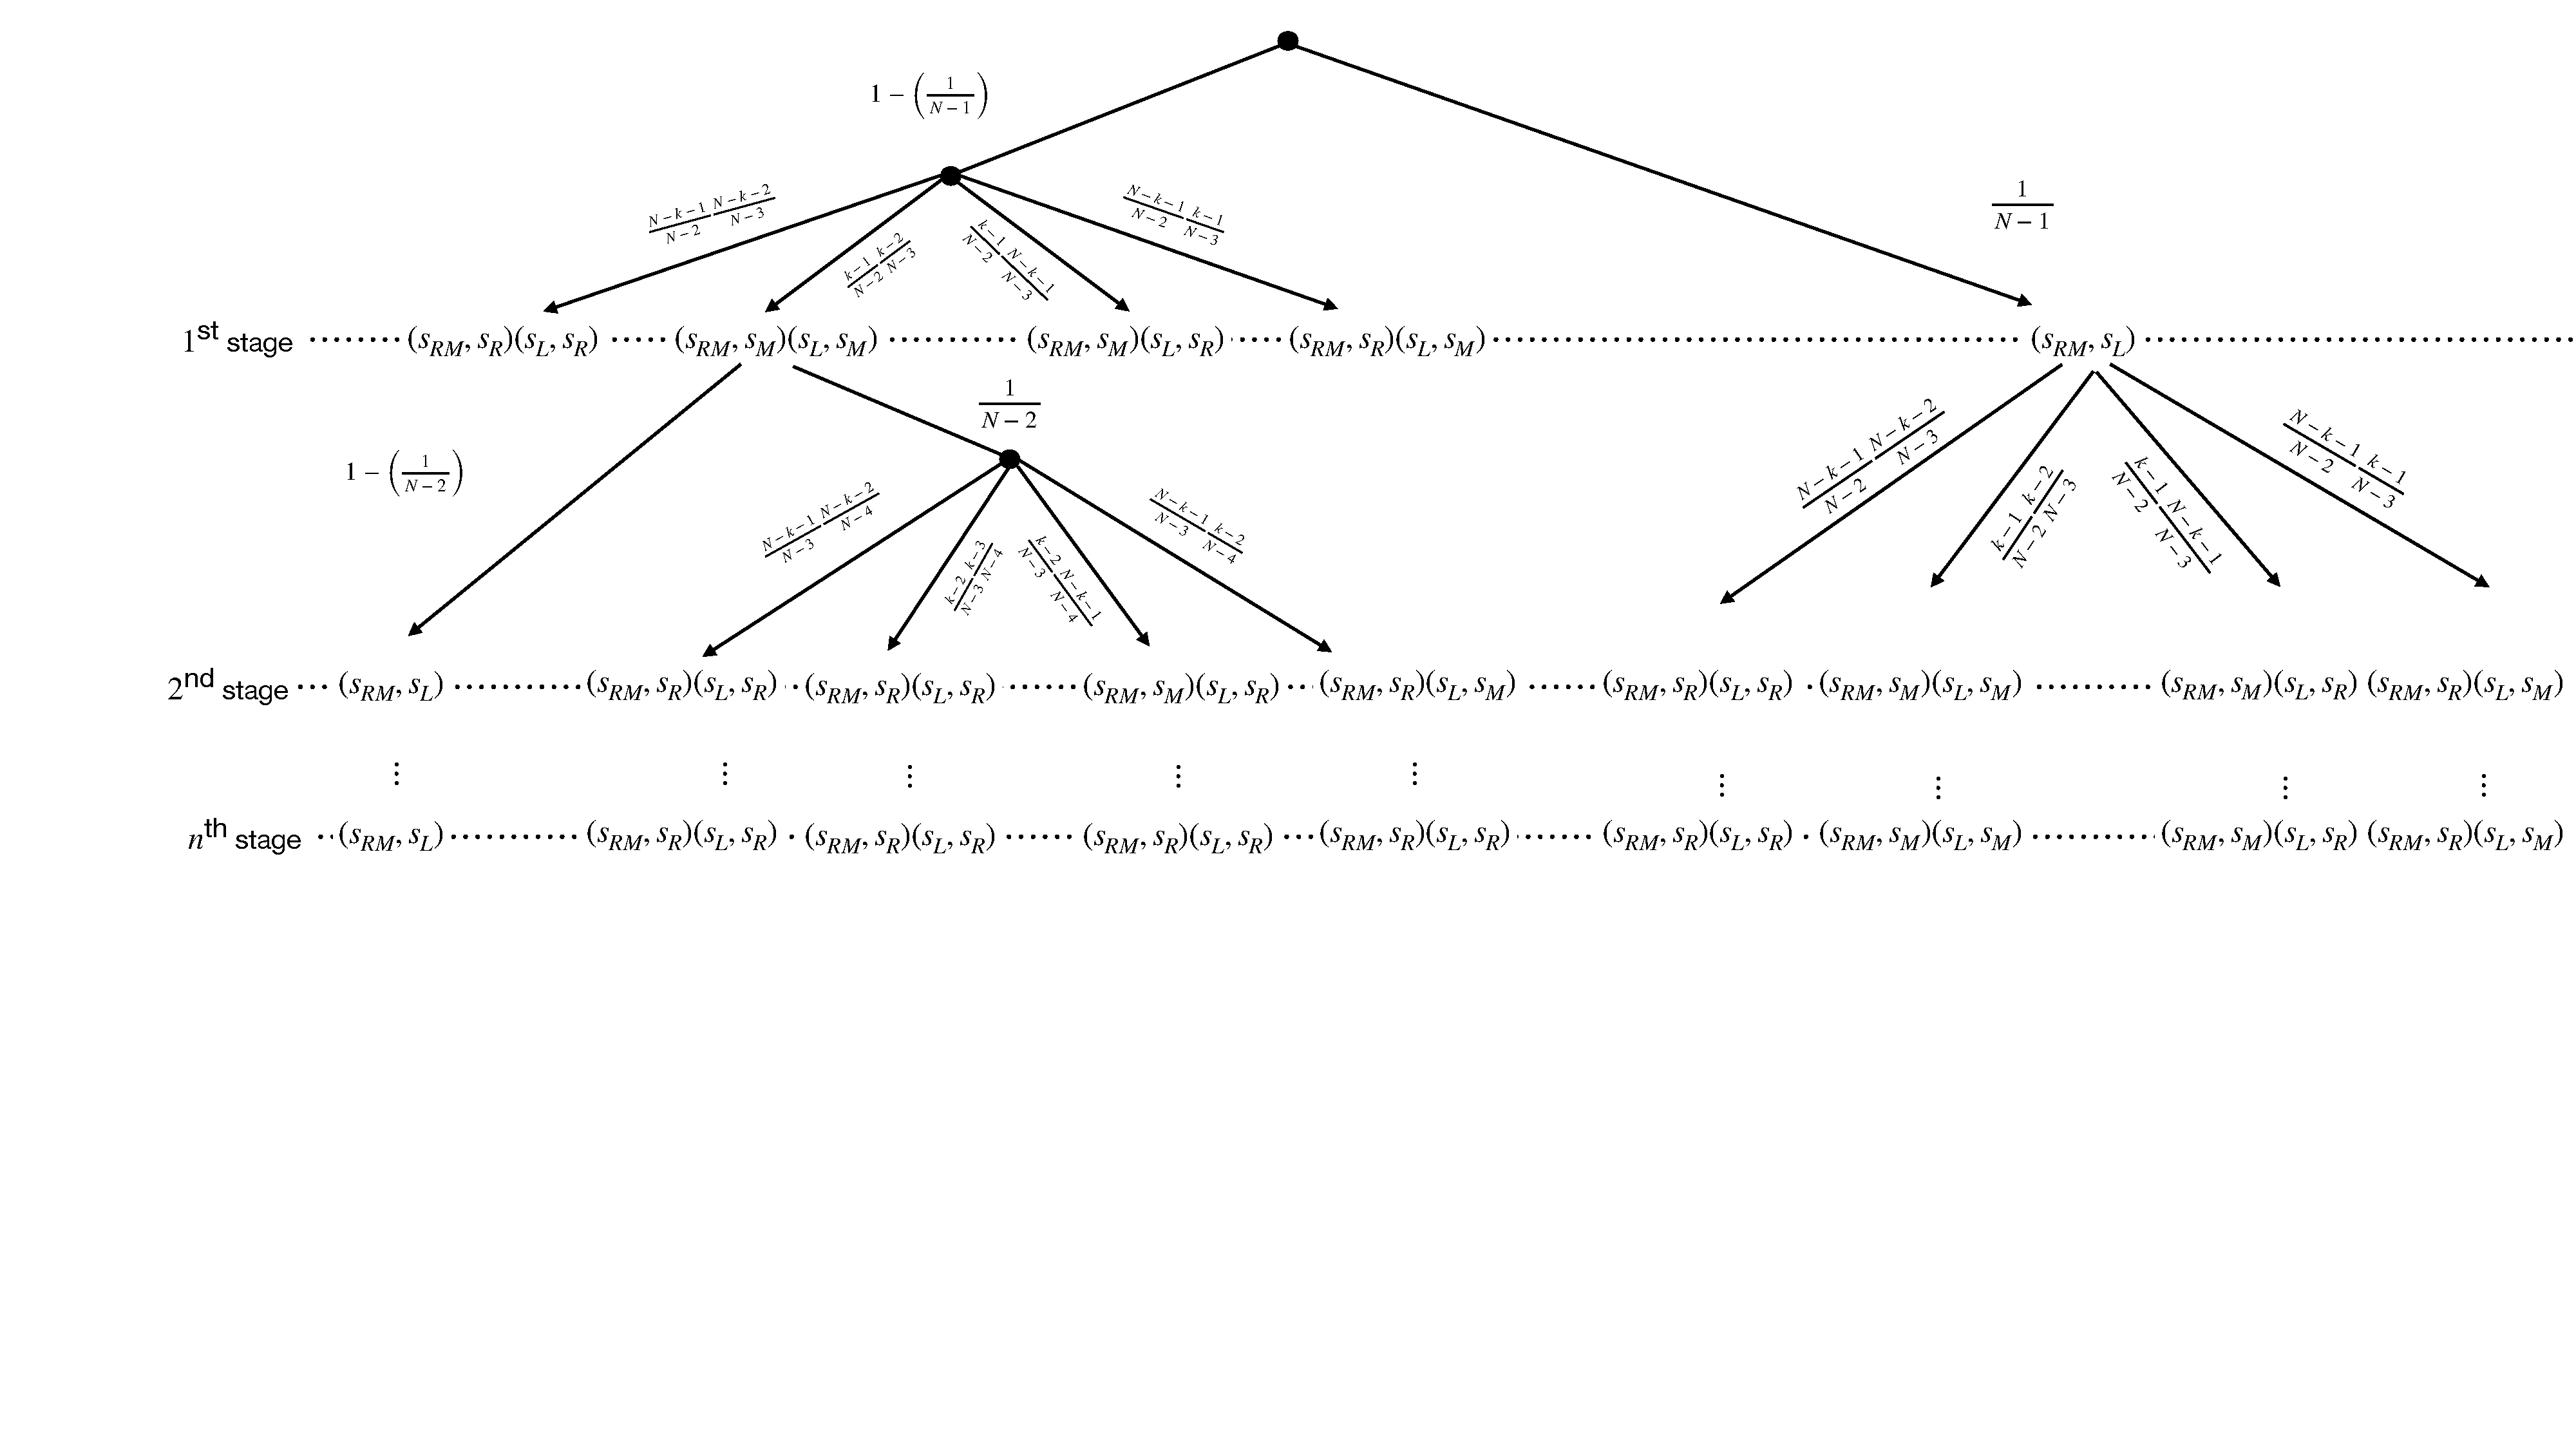
\includegraphics[width=\textwidth]{static/matching_tree.pdf}
  \caption{\textbf{Tree diagram of the possible pairs when the learner and the role
  model have $n$ interactions.} In the diagram \((s_i, s_j)\) represent a possible
  pair. We denote the role model as $s_{RM}$ and the learner as $s_{L}$, and
  a member of the population that plays a mutant strategy is denoted as $s_{M}$ and
  a resident strategy as $s_{R}$. The role model and
  the learner need to be paired with $n$ other members of the population
  (including each other). We break down the process into stages. For the first
  pair (stage one) the role model and the mutant can be paired together (with
  probability $\frac{1}{N-1}$) or not (with probability $1 -
  \left(\frac{1}{N-1}\right)$). In the case that they are not paired together,
  both can be paired with a mutant $\frac{(k-1)(k-2)}{(N-2)(N-3)}$, with a
  resident $\frac{(N-k-1)(N-k-2)}{(N-2)(N-3)}$, or one is paired with a mutant
  whilst the other is paired with a resident $\frac{(N-k-1)(k-1)}{(N-2)(N-3)}$.
  There are five possible pairs for stage one as we have already discussed
  in Section~\ref{section:limited_memory}. In
  the second stage we need to consider if the role model and the learner
  interacted with each other. If yes, then they can not interact with each other
  again, and at each stage there are at most four possible pairs; they interact with
  mutants, with residents, or the one interacts with a mutant whilst the second
  interacts with a resident. In the case that they were not paired in stage 1
  there are five possible pairs. These pairs are the same as in stage 1,
  however now the probabilities differ. Namely, let's assume that in the
  first stage both were matched with a mutant. They interact with each
  other with a probability $\frac{1}{N-2}$ or not with a probability
  $1 - \left(\frac{1}{N-2}\right)$. In the latter case there are four
  possible pairs.
  Both can be paired with a mutant $\frac{(k-1)(k-2)}{(N-3)(N-4)}$, with a
  resident $\frac{(N-k-1)(N-k-2)}{(N-3)(N-4)}$, or one is paired with a mutant
  whilst the other is paired with a resident $\frac{(N-k-1)(k-2)}{(N-3)(N-4)}$.
  The process continues following the same logic until it reaches the $n^{\text{th}}$
  stage.}\label{fig:matching_tree}
\end{figure}

\subsubsection{Last Round Payoff of Two Interactions}

Here the learner and role model consider the last round payoff of two
interactions. At each time step of the evolutionary process there are twenty
four possible pairs. At the first stage there are fiver possible pairs. For four of
these pairs there are five possible pairs in the second stage (\(4 \times 5 =
20\)), and for the last one there are four possible pairs in the second stage
(20 + 4 = 24). 

We assume that player \(s_1\) receives the payoff
\(u_{11}\) with their first interaction and \(u_{12}\) with their second.
Respectively, player \(s_2\) receives \(u_{21}\) and \(u_{22}\). We define the
probability that the respective last round payoffs of the two players \(s_1,
s_2\) are given by \((u_{11}, u_{11})\) and \((u_{21}, u_{22})\) as
\(x^{2}((u_{11}, u_{11}), (u_{21}, u_{22}))\) given by,

\begin{equation}
  \resizebox{.99\textwidth}{!}
  {%
$
  \setlength{\arraycolsep}{1pt}
  \begin{array}{llrl}
  x^{2}((u_{11}, u_{12}), (u_{21}, u_{22}))	& = \displaystyle \frac{1}{N\!-\!1}\cdot v_{u_{11}}(s_1,s_2)\cdot 1_{(u_{11},u_{21})\in \mathcal{U}_F} \cdot A + \left(1\!-\!\frac{1}{N\!-\!1}\right) \left[ \right. \\[0.5cm] 
  & \left. v_{u_{11}}(s_1,s_2) _{u_{21}}(s_2,s_2)  \frac{\left(k - 2\right) \left(k - 1\right)}{(N\!-\!2)(N\!-\!3)}
  \left(\frac{1}{N\!-\!2}\cdot v_{u_{11}}(s_1,s_2)\cdot 1_{(u_{11},u_{21})\in \mathcal{U}_F} + (1 - \frac{1}{N - 2}) [B_1 + B_2 + B_3 + B_4]\right) + \right. \\[0.5cm] 
  & \left. v_{u_{11}}(s_1,s_2) _{u_{21}}(s_2,s_1)  \frac{\left(k - 1\right) \left(N - k - 1\right)}{(N\!-\!2)(N\!-\!3)} \left(\frac{1}{N\!-\!2}\cdot v_{u_{11}}(s_1,s_2)\cdot 1_{(u_{11},u_{21})\in \mathcal{U}_F} + (1 - \frac{1}{N - 2}) [C_1 + C_2 + C_3 + C_4]\right) + \right. \\[0.5cm] 
  & \left. v_{u_{11}}(s_1,s_1) _{u_{21}}(s_2,s_2)  \frac{\left(k - 1\right) \left(N - k - 1\right)}{(N\!-\!2)(N\!-\!3)} \left(\frac{1}{N\!-\!2}\cdot v_{u_{11}}(s_1,s_2)\cdot 1_{(u_{11},u_{21})\in \mathcal{U}_F} + (1 - \frac{1}{N - 2}) [D_1 + D_2 + D_3 + D_4]\right) + \right. \\[0.5cm] 
  & \left. v_{u_{11}}(s_1,s_1) _{u_{21}}(s_2,s_1)  \frac{\left(N - k - 2\right) \left(N - k - 1\right)}{(N\!-\!2)(N\!-\!3)} \left(\frac{1}{N\!-\!2}\cdot v_{u_{11}}(s_1,s_2)\cdot 1_{(u_{11},u_{21})\in \mathcal{U}_F} + (1 - \frac{1}{N - 2}) [E_1 + E_2 + E_3 + E_4]\right) \right]
  \end{array} $}
\end{equation}

\begin{equation}
  \resizebox{.9\textwidth}{!}
  {%
$
  \setlength{\arraycolsep}{1pt}
  \begin{array}{llrl}
  A & = \left(1\!-\!\frac{1}{N\!-\!1}\right)  \left[ \frac{k\!-\!1}{N\!-\!2}\frac{k\!-\!2}{N\!-\!3} v_{u_{21}}(s_1,s_2) v_{u_{22}}(s_2,s_2) + 
   \frac{k\!-\!1}{N\!-\!2}\frac{N\!-\!k\!-\!1}{N\!-\!3} v_{u_{21}}(s_1,s_2) v_{u_{22}}(s_2,s_1) + \right. \\[0.5cm]
   & \left. \frac{N\!-\!k\!-\!1}{N\!-\!2}\frac{k\!-\!1}{N\!-\!3} v_{u_{21}}(s_1,s_1) v_{u_{22}}(s_2,s_2) + 
   \frac{N\!-\!k\!-\!1}{N\!-\!2}\frac{N\!-\!k\!-\!2}{N\!-\!3} v_{u_{21}}(s_1,s_1) v_{u_{22}}(s_2,s_1)\right] \\[0.5cm] 
   B_1 & = \frac{\left(k - 3\right) \left(k - 2\right)}{(N - 3) (N - 4)} v_{u_{21}}(s_1,s_2) v_{u_{22}}(s_2,s_2) \quad
   B_2 = \frac{\left(k - 2\right) \left(N - k - 1\right)}{(N - 3) (N - 4)} v_{u_{21}}(s_1,s_1) v_{u_{22}}(s_2,s_2) \\[0.5cm] 
   B_3 & = \frac{\left(k - 2\right) \left(N - k - 1\right)}{(N - 3) (N - 4)} v_{u_{21}}(s_1,s_2) v_{u_{22}}(s_2,s_1) \quad
   B_4 = \frac{\left(N - k - 2\right) \left(N - k - 1\right)}{(N - 3) (N - 4)} v_{u_{21}}(s_1,s_1) v_{u_{22}}(s_2,s_1) \\[0.5cm] 

   C_1 & = \frac{\left(k - 3\right) \left(k - 1\right)}{(N - 3) (N - 4)} v_{u_{21}}(s_1,s_2) v_{u_{22}}(s_2,s_2) \quad
   C_2 = \frac{\left(k - 1\right) \left(N - k - 1\right)}{(N - 3) (N - 4)} v_{u_{21}}(s_1,s_1) v_{u_{22}}(s_2,s_2) \\[0.5cm] 
   C_3 & = \frac{\left(k - 2\right) \left(N - k - 2\right)}{(N - 3) (N - 4)} v_{u_{21}}(s_1,s_2) v_{u_{22}}(s_2,s_1) \quad
   C_4 = \frac{\left(N - k - 2\right)^{2}}{(N - 3) (N - 4)} v_{u_{21}}(s_1,s_1) v_{u_{22}}(s_2,s_1) \\[0.5cm] 

   D_1 & = \frac{\left(k - 2\right)^{2}}{(N - 3) (N - 4)} v_{u_{21}}(s_1,s_2) v_{u_{22}}(s_2,s_2) \quad
   D_2 = \frac{\left(k - 2\right) \left(N - k - 2\right)}{(N - 3) (N - 4)} v_{u_{21}}(s_1,s_1) v_{u_{22}}(s_2,s_2) \\[0.5cm] 
   D_3 & = \frac{\left(k - 1\right) \left(N - k - 1\right)}{(N - 3) (N - 4)} v_{u_{21}}(s_1,s_2) v_{u_{22}}(s_2,s_1) \quad
   D_4 = \frac{\left(N - k - 3\right) \left(N - k - 1\right)}{(N - 3) (N - 4)} v_{u_{21}}(s_1,s_1) v_{u_{22}}(s_2,s_1) \\[0.5cm]

   E_1 & = \frac{\left(k - 2\right) \left(k - 1\right)} v_{u_{21}}(s_1,s_2) v_{u_{22}}(s_2,s_2) \quad
   E_2 = \frac{\left(k - 1\right) \left(N - k - 2\right)}{(N - 3) (N - 4)} v_{u_{21}}(s_1,s_1) v_{u_{22}}(s_2,s_2) \\[0.5cm] 
   E_3 & = \frac{\left(k - 1\right) \left(N - k - 2\right)}{(N - 3) (N - 4)} v_{u_{21}}(s_1,s_2) v_{u_{22}}(s_2,s_1) \quad
   E_4 = \frac{\left(N - k - 3\right) \left(N - k - 2\right)}{(N - 3) (N - 4)} v_{u_{21}}(s_1,s_1) v_{u_{22}}(s_2,s_1) \\[0.5cm] 
  \end{array}$}
\end{equation}

The first term on the right side corresponds to the case that the learner and
the role model happened to be matched during the first stage,
followed by them being paired with another member of the population on the
second stage. The second terms corresponds to the case that the learner and the
role model interact with a mutant with a probability ($\frac{\left(k - 2\right)
\left(k - 1\right)}{(N\!-\!2)(N\!-\!3)}$). In the seconds stage, they can either
interact with each other $\frac{1}{N - 2}$ or not $(1 - \frac{1}{N - 2})$. If
they do not interact with each other, then each of the following can happen:
both of them interact with a mutant with a probability
$\frac{(k-3)(k-2)}{(N-4)(N-3)}$ and both interact with a resident with a
probability $\frac{(N-k-1)(N-k-2)}{(N-3)(N-4)}$. The last two possible pairs
are that either of them interacts with a resident whilst the other interacts
with a mutant, and this happens with a probability
$\frac{(N-k-2)(k-1)}{(N-4)(N-3)}$, and so on.

The probability that the number of mutants increases, and decreases
respectively, by one is now given by,

\begin{align}\label{eq:ratio_limited}
\lambda^+_k=\frac{N\!-\!k}{N}\cdot \frac{k}{N}\cdot \sum_{u_{R1},u_{M1}\in\mathcal{U}} \quad \sum_{u_{R2},u_{M2}\in\mathcal{U}} x^{2}((u_{R1}, u_{R2}),(u_{M1}, u_{M2}))\cdot \rho\left(\frac{u_{R1} + u_{R2}}{2}, \frac{u_{M1} + u_{M2}}{2}\right), \\
\lambda^-_k=\frac{N\!-\!k}{N}\cdot \frac{k}{N}\cdot \sum_{u_{R1},u_{M1}\in\mathcal{U}} \quad \sum_{u_{R2},u_{M2}\in\mathcal{U}} x^{2}((u_{R1}, u_{R2}),(u_{M1}, u_{M2}))\cdot \rho\left(\frac{u_{M1} + u_{M2}}{2}, \frac{u_{R1} + u_{R2}}{2}\right).
\end{align}

We use $x^{2}((u_{R1}, u_{R2}),(u_{M1}, u_{M2}))$ to denote the probability that
the randomly chosen resident obtained a payoff of $u_{R1}$ in the last round of
their first respective game and $u_{R1}$ in the last round of their second game.
Similarly, that the mutant obtained a payoff of $u_{M1}$ from their first
interaction and $u_{M2}$ from the second. Note that we assume that the players
compare their average payoff of their two interaction when considering adopting
the others strategy. For example the mutant adopts the resident's strategy with
a probability $\rho\left(\frac{u_{R1} + u_{R2}}{2}, \frac{u_{M1} +
u_{M2}}{2}\right)$.

~\\
{\bf Invasion Analysis}

In a similar fashion we can calculate the condition for which a population of
GTFT players can not be invaded by an ALLD mutant. Using the new formulation we
obtain the following probabilities \(x^{2}((u_{11}, u_{12}), (u_{21}, u_{22}))\) that the payoff of a randomly
chosen GTFT player is \((u_{11}, u_{12})\) and that the payoff of the ALLD player is \((u_{21}, u_{22})\),

\begin{align*}
  x^{2}((r, r), (t, t)) = & \frac{N - 3}{N - 1}\left(\delta q - \delta + 1\right)^{2} & 
  x^{2}((r, r), (t, p)) = & - \frac{N - 3}{N - 1} \delta \left(q - 1\right) \left(\delta q - \delta + 1\right)\\
  x^{2}((r, r), (p, t)) = & - \frac{N - 3}{N - 1} \delta \left(q - 1\right) \left(\delta q - \delta + 1\right) &
  x^{2}((r, r), (p, p)) = & \frac{N - 3}{N - 1} \delta^{2}  \left(q - 1\right)^{2}\\
  x^{2}((r, s), (t, t)) = & \frac{1}{N-1} \left(\delta q - \delta + 1\right)^{2} &
  x^{2}((r, s), (p, t)) = & - \frac{1}{N-1} \delta \left(q - 1\right) \left(\delta q - \delta + 1\right) \\
  x^{2}((r, p), (t, p)) = & - \frac{1}{N-1} \delta \left(q - 1\right) \left(\delta q - \delta + 1\right) &
  x^{2}((r, p), (p, p)) = & \frac{1}{N-1} \delta^{2} \left(q - 1\right)^{2} \\
  x^{2}((s, r), (t, t)) = & \frac{1}{N-1} \left(\delta q - \delta + 1\right)^{2} &
  x^{2}((s, r), (t, p)) = & - \frac{1}{N-1} \delta \left(q - 1\right) \left(\delta q - \delta + 1\right)\\
  x^{2}((p, r), (p, t)) = & - \frac{1}{N-1} \delta \left(q - 1\right) \left(\delta q - \delta + 1\right) &
  x^{2}((p, r), (p, p)) = & \frac{1}{N-1} \delta^{2} \left(q - 1\right)^{2} \\
  x^{2}((u_{11}, u_{12}), (u_{21}&, u_{22})) =  0 \text{ for all other payoff pairs} & ((u_{11}, u_{12}), (u_{21}, u_{22})). &
\end{align*}

The ratio of transition probabilities is given by,

\begin{equation}
  \resizebox{.9\textwidth}{!}
  {%
$\frac{\lambda^{+}}{\lambda^{-}} =
\frac{\frac{N - 3}{N-1} \left(\frac{\delta^{2} \left(1 - q\right)^{2}}{1 + e^{- \beta \left(- b + c\right)}} + \frac{2 \delta \left(1 - q\right) \left(\delta q - \delta + 1\right)}{1 + e^{- \beta \left(- \frac{b}{2} + c\right)}} + \frac{\left(\delta q - \delta + 1\right)^{2}}{1 + e^{- \beta c}}\right) 
+ \frac{2}{N-1} \left(\frac{\delta^{2} \left(1 - q\right)^{2}}{1 + e^{- \beta \left(- \frac{b}{2} + \frac{c}{2}\right)}} + \frac{\delta \left(1 - q\right) \left(\delta q - \delta + 1\right)}{1 + e^{- \frac{\beta c}{2}}} + \frac{\delta \left(1 - q\right) \left(\delta q - \delta + 1\right)}{1 + e^{- \beta c}} + \frac{\left(\delta q - \delta + 1\right)^{2}}{1 + e^{- \beta \left(\frac{b}{2} + c\right)}}\right)}
{\frac{N - 3}{N-1} \left(\frac{\delta^{2} \left(q - 1\right)^{2}}{1 + e^{- \beta \left(b - c\right)}} + \frac{2 \delta \left(1 - q\right) \left(\delta q - \delta + 1\right)}{1 + e^{- \beta \left(\frac{b}{2} - c\right)}} + \frac{\left(\delta q - \delta + 1\right)^{2}}{e^{\beta c} + 1}\right) + \frac{2}{N-1} \left(\frac{\delta^{2} \left(q - 1\right)^{2}}{1 + e^{- \beta \left(\frac{b}{2} - \frac{c}{2}\right)}} + \frac{\delta \left(1 - q\right) \left(\delta q - \delta + 1\right)}{e^{\beta c} + 1} + \frac{\delta \left(1 - q\right) \left(\delta q - \delta + 1\right)}{e^{\frac{\beta c}{2}} + 1} + \frac{\left(\delta q - \delta + 1\right)^{2}}{1 + e^{- \beta \left(- \frac{b}{2} - c\right)}}\right)}
$}
\end{equation}

In the limit of strong selection \(\beta \rightarrow \infty\) and large
populations \(N \rightarrow \infty \) we obtain the following cases,

\begin{equation}
\frac{\lambda^{+}}{\lambda^{-}} = 
\begin{cases}
  - \frac{q \left(\delta q - \delta + 1\right)}{\left(q - 1\right) \left(\delta q + 1\right)}  & \frac{b}{2} > c \\[0.5cm]
  \frac{- \delta q + \delta - 1}{\delta \left(q - 1\right)}  & \frac{b}{2} = c \\[0.5cm]
  - \frac{\delta q^{2} - 2 \delta q + \delta - 1}{\delta \left(q - 1\right)^{2}} & \frac{b}{2} < c
\end{cases}
\end{equation}

We note that the relationship between the cost and benefit have an effect on how
generous a conditional cooperator must be to avoid invasion. In the case of
\(\frac{b}{2}=c\) the result remains the same expression as in the case of
\(m=n=1\). For the other two cases we show that for
\(\frac{\lambda^{+}}{\lambda^{-}} < 1\),

\begin{equation}
\begin{cases}
  q < \left\{\frac{\delta - 1 - \frac{\sqrt{2}}{2}}{\delta}, \frac{\delta - 1 + \frac{\sqrt{2}}{2}}{\delta}\right\}  & \frac{b}{2} > c \\[0.5cm]
  q < \left\{\frac{\delta - \frac{\sqrt{2}}{2}}{\delta}, \  \frac{\delta + \frac{\sqrt{2}}{2}}{\delta}\right\} & \frac{b}{2} < c
\end{cases}
\end{equation}

For \(\frac{b}{2}>c\) the ratio is smaller for \(q < \left\{\frac{\delta - 1 -
\frac{\sqrt{2}}{2}}{\delta}, \frac{\delta - 1 +
\frac{\sqrt{2}}{2}}{\delta}\right\}\), however, \(\frac{\delta - 1 -
\frac{\sqrt{2}}{2}}{\delta}\) is not a feasible root since it's always smaller
than 1, and thus \(q < \frac{\delta - 1 + \frac{\sqrt{2}}{2}}{\delta}\). For
infinitely repeated games, \(\delta \rightarrow 1\), this condition becomes \(q
< \frac{\sqrt{2}}{2}\). In the case of \(\frac{b}{2}<c\) there are two possible
roots. For repeated games that are repeated for a large number of turn such as
\(\delta \rightarrow 1\) the condition then becomes \(q < 1 -
\frac{\sqrt{2}}{2}\).

\subsection{Updating Payoffs based on the Last $m$ Rounds Payoffs of One Interaction}\label{section:m_two_n_one}

The second generalised case of the limited memory payoffs we discuss is that of
individuals updating based on their last $m$ rounds payoffs with one member. Let
\(\mathcal{U}^{m}= \{\underbrace{rrr\dots r}_{m}, \underbrace{rrr\dots s}_{m},
\dots, \underbrace{ppp\dots p}_{m}\}\) be the set of feasible payoffs of the
last $m$ rounds. The probability that a reactive strategy receives the payoffs
$u\!\in\! \mathcal{U}^{m}$ is given by
Proposition~\ref{proposition:last_m_rounds}.

\begin{Prop}\label{proposition:last_m_rounds} Consider a repeated game, with
  continuation probability $\delta$, between players with reactive strategies
  $s_1\!=\!(y_1, p_1, q_1$) and $s_2\!=\!(y_2,p_2,q_2)$ respectively. Let
  $\mathcal{U}^{m}$ denote the set of feasible payoffs in the last
  \(m\) rounds, and let \(\mathbf{u}^{m}\) be the corresponding payoff vector.
  Then the probability that the $s_1$ player receives the payoff $u\!\in\!
  \mathcal{U}^{m}$ in the very last two rounds of the game is given by,

  \begin{equation}
  \langle\mathbf{v}^{m}(s_1,s_2),\mathbf{u}^{m}\rangle, \text{ where } \mathbf{v}^{m} \in R^{4^{m}} \text{ is given by },
  \end{equation}
  \begin{equation}
    \mathbf{v}^{m}(s_1,s_2) = (1 - \delta) w_{a_1, a_2} \delta^2 \left[\mathbf{v_0}(I_4 - \delta M)^{-1}\right]_{a_1, a_2}, \quad  w_{a_1, a_2} \in M \ \forall \ a_1, a_2 \in \{1, 2, 3, 4\}.
  \end{equation}
\end{Prop}

\subsubsection{Last Round Payoff of Two Interactions}

In the special case of $m=2$ the stationary distribution \(\mathbf{v}^{2}(s_1,
s_2)\) is sixteen dimension instead of four dimensional where \(v_{1}(s_1, s_2)\) is
the long term probability that \(s_1\) and \(s_2\) mutually cooperated in the
last two rounds. Let the feasible payoffs a strategy can receive
be $\mathcal{U}^{2} = \{rr, rs, rt, rp, sr, \dots, pp\}$.
The role model and the learner interact with only one other member and so the
probability \(x\) remains the same as in Section~\ref{section:limited_memory}.

The probability that the number of mutants increases, and decreases respectively,
by one is now given by,

\begin{align}
\lambda^+_k=\frac{N\!-\!k}{N}\cdot \frac{k}{N} \cdot \sum_{u_{R},u_{M}\in\mathcal{U}^{2}} x(u_{R},u_{M})\cdot \rho\left(\frac{u_{R}}{2},\frac{u_{M}}{2}\right), \\
\lambda^-_k=\frac{N\!-\!k}{N}\cdot \frac{k}{N} \cdot \sum_{u_{R},u_{M}\in\mathcal{U}^{2}} x(u_{R},u_{M})\cdot \rho\left(\frac{u_{M}}{2},\frac{u_{R}}{2}\right).
\end{align}

We assume again that players consider their average payoff of the last two turns
when deciding to imitate another strategy or not.

~\\
{\bf Invasion Analysis}

We once again calculate how easily a single ALLD mutant can invade into a
resident population of GTFT player. When two GTFT players interact in the game,
their respective probabilities for each of the four outcomes in the last round
simplify to,

\begin{align*}
    v_{rr}(GTFT,GTFT) = & \delta^2, \text{ and }\\
    v_{i}(GTFT,GTFT) = &  0 \text{ for all other } i \in \mathcal{U}^{2}.
\end{align*}

On the other hand, if an ALLD player interacts with a GTFT player, the
respective probabilities according to Eq.~\ref{Eq:LastRound} become

\begin{align*}
    v_{tt} (ALLD,GTFT) & = \delta^{2} q \left(\delta q - \delta + 1\right), & 
    v_{tp}(ALLD,GTFT) & = - \delta^{2} \left(q - 1\right) \left(\delta q - \delta + 1\right), \\
    v_{pt} (ALLD, GTFT ) & = \delta^{3} q \left(1 - q\right), & 
    v_{pp} (ALLD, GTFT) & = \delta^{3} \left(q - 1\right)^{2} \text{ and }\\
    v_{i}(ALLD,GTFT) & =  0 \text{ for all other } i \in \mathcal{U}^{2}.
\end{align*}

As a consequence, we obtain the following probabilities \(x(u_1, u_2)\) that the
payoff of a randomly chosen GTFT player is \(u_1\) and that the payoff of the
ALLD player is \(u_2\),

\begin{align*}
  x(rr, tt) = & \frac{N-2}{N - 1} \delta^{4} q \left(N - 2\right) \left(\delta q - \delta + 1\right) &
  x(rr, tp) = & - \frac{N-2}{N - 1} \delta^{4} \left(N - 2\right) \left(q - 1\right) \left(\delta q - \delta + 1\right)\\
  x(rr, pt) = & - \frac{N-2}{N - 1} \delta^{5} q \left(N - 2\right) \left(q - 1\right) &
  x(rr, pp) = & \frac{N-2}{N - 1} \delta^{5} \left(N - 2\right) \left(q - 1\right)^{2}\\
  x(ss, tt) = & \frac{1}{N -1}\delta^{2} q \left(\delta q - \delta + 1\right) & 
  x(sp, tp) = & - \frac{1}{N -1}\delta^{2} \left(q - 1\right) \left(\delta q - \delta + 1\right) \\
  x(ps, pt) = & - \frac{1}{N -1}\delta^{3} q \left(q - 1\right) &
  x(pp, pp) = & \frac{1}{N -1}\delta^{3} \left(q - 1\right)^{2}\\
  x(u_1, u_2) = &  0 \text{ for all other payoff pairs } (u_1, u_2). &
\end{align*}

We now calculate the ratio of transition probabilities as

\begin{equation}
  \resizebox{.9\textwidth}{!}
  {%
  $\frac{\lambda^{+}}{\lambda^{-}} =
  \frac{\frac{\delta^{2} \left(N - 2\right)}{N-1} \left(\frac{\delta \left(1 - q\right)^{2}}{1 + e^{- \beta \left(- b + c\right)}} + \frac{q \left(\delta q - \delta + 1\right)}{1 + e^{- \beta c}} + \frac{\left(1 - q\right) \left(2 \delta q - \delta + 1\right)}{1 + e^{- \beta \left(- \frac{b}{2} + c\right)}}\right) + \frac{1}{N-1}\left(\frac{\delta \left(1 - q\right)^{2}}{2} + \frac{q \left(\delta q - \delta + 1\right)}{1 + e^{- \beta \left(b + c\right)}} + \frac{\left(1 - q\right) \left(2 \delta q - \delta + 1\right)}{1 + e^{- \beta \left(\frac{b}{2} + \frac{c}{2}\right)}}\right)}
  {\frac{\delta^{2} \left(N - 2\right)}{N-1} \left(\frac{\delta \left(1 - q\right)^{2}}{1 + e^{- \beta \left(b - c\right)}} + \frac{q \left(\delta q - \delta + 1\right)}{e^{\beta c} + 1} + \frac{\left(1 - q\right) \left(2 \delta q - \delta + 1\right)}{1 + e^{- \beta \left(\frac{b}{2} - c\right)}}\right) + \frac{1}{N-1} \left(\frac{\delta \left(1 - q\right)^{2}}{2} + \frac{q \left(\delta q - \delta + 1\right)}{1 + e^{- \beta \left(- b - c\right)}} + \frac{\left(1 - q\right) \left(2 \delta q - \delta + 1\right)}{1 + e^{- \beta \left(- \frac{b}{2} - \frac{c}{2}\right)}}\right)}
  $}
\end{equation}

In the limit of strong selection \(\beta \rightarrow \infty\) and large
populations \(N \rightarrow \infty \) we obtain three expressions depending on
the cost-benefit relationship. We note that for \(\frac{b}{2}=c\) the result
remains the same expression as in the case of \(m=n=1\).

\begin{equation}
\frac{\lambda^{+}}{\lambda^{-}} = 
\begin{cases}
  - \frac{q \left(\delta q - \delta + 1\right)}{\left(q - 1\right) \left(\delta q + 1\right)}  & \frac{b}{2} > c \\[0.5cm]
  - \frac{\delta q - \delta + q + 1}{\left(\delta + 1\right) \left(q - 1\right)}  & \frac{b}{2} = c \\[0.5cm]
  - \frac{\delta q^{2} - 2 \delta q + \delta - 1}{\delta \left(q - 1\right)^{2}} & \frac{b}{2} < c
\end{cases}
\end{equation}

For \(\frac{\lambda^{+}}{\lambda^{-}} < 1\):

\begin{equation}
\begin{cases}
  q \in \left\{\frac{\delta - \sqrt{\delta^{2} + 1} - 1}{2 \delta}, \  \frac{\delta + \sqrt{\delta^{2} + 1} - 1}{2 \delta}\right\}  & \frac{b}{2} > c \\[0.5cm]
  q \in \left\{1 - \frac{\sqrt{2}}{2 \sqrt{\delta}}, \  1 + \frac{\sqrt{2}}{2 \sqrt{\delta}}\right\} & \frac{b}{2} < c
\end{cases}
\end{equation}

For \(\frac{b}{2}>c\) the ratio is smaller for
\(q < \left\{\frac{\delta - \sqrt{\delta^{2} + 1} - 1}{2 \delta}, \frac{\delta + \sqrt{\delta^{2} + 1} - 1}{2 \delta}\right\}\)
, however, the first root is not a feasible root since it's always smaller
than 1, and thus \(q < \frac{\delta + \sqrt{\delta^{2} + 1} - 1}{2 \delta}\). For
infinitely repeated games, \(\delta \rightarrow 1\), this condition becomes \(q
< \frac{\sqrt{2}}{2}\). In the case of \(\frac{b}{2}<c\) there are two possible
roots. For repeated games that are repeated for a large number of turn such as
\(\delta \rightarrow 1\) the condition then becomes \(q < 1 -
\frac{\sqrt{2}}{2}\).

Note that as \(\delta \rightarrow 1\) the condition for which condition
cooperators can avoid invasion is the same for the case of \(m=2\) and \(n=2\).

\subsection{Updating Payoffs based on the last two rounds payoff of two interactions (\(m=2\) and \(n=2\))}\label{section:m_two_n_two}

The final extension to the limited memory framework we consider is that of
increasing the number of rounds and the number of interactions. For this case we
need to consider a combination of the methods we presented in
Section~\ref{section:m_one_n_two} and Section~\ref{section:m_two_n_one}. As an
example consider the case of \(m=n=2\). The probability that the number of
mutants increases, and decreases respectively, by one is now given by,

\begin{align}
  \lambda^+_k=\frac{N\!-\!k}{N}\cdot \frac{k}{N}\cdot \sum_{u_{R1},u_{M1}\in\mathcal{U}^{2}} \quad \sum_{u_{R2},u_{M2}\in\mathcal{U}^{2}} x^{2}((u_{R1}, u_{R2}),(u_{M1}, u_{M2}))\cdot \rho\left(\frac{u_{R1} + u_{R2}}{2}, \frac{u_{M1} + u_{M2}}{2}\right), \\
  \lambda^-_k=\frac{N\!-\!k}{N}\cdot \frac{k}{N}\cdot \sum_{u_{R1},u_{M1}\in\mathcal{U}^{2}} \quad \sum_{u_{R2},u_{M2}\in\mathcal{U}^{2}} x^{2}((u_{R1}, u_{R2}),(u_{M1}, u_{M2}))\cdot \rho\left(\frac{u_{M1} + u_{M2}}{2}, \frac{u_{R1} + u_{R2}}{2}\right).
\end{align}

Though we do not carry any further analytical exploration of this case, in the
next section we present simulation results when the updating payoffs of the
pairwise process depend on the limited memory framework with \(m=n=2\), as well
as the rest of the cases we have discussed so far.


%%%%%%%%%%%%%%%%%%
%% FURTHER SIMULATIONS %% 
%%%%%%%%%%%%%%%%%%

\section{Further simulation results}~\label{section:furthersimulations}


\subsection{Simulation Results on the Pairwise Comparison Process}\label{section:simulation_results}

We simulate the evolutionary process described in
Algorithm~\ref{algorithm:pairwise_comparison} for the different updating
mechanisms we have described in
Sections~\ref{section:perfect_memory}-\ref{section:m_two_n_two}. For each
approach we performed an independent run of the process and for each time step we
recorded the current resident population \((y, p, q)\). The results are shown in
Figure~\ref{fig:expected_payoffs_results}. We observe that in most cases the
resident population consists either of defectors or conditional cooperators. A
conditional cooperator always cooperates if the co-player cooperated
($p\approx1$) and cooperates with a probability \(q\) if the co-player defected.
The most abundant conditional cooperators in each simulation differ as a
result of the updating payoffs. More specifically, in order for a resident
population of conditional cooperators to avoid being invaded they need to adopt
a different value of \(q\). For each method we have discussed this under the
invasion analysis subsection. 

In the cases of perfect memory the resident population adopts a \(q \leq 1 -
\frac{c}{b}=0.9\). In the limited memory case the generosity of a conditional
cooperator is independently of the benefit lower than \(\frac{1}{2}\). The rest
of the cases also condition on the cost benefit relationship. In these
simulations the cost of cooperation is set to 1 and the benefit to 10. As a
result, in the case of two interactions \(q \leq \frac{\delta - 1 +
\frac{\sqrt{2}}{2}}{\delta}=0.7068\), in the case of two rounds \(q \leq
\frac{\delta + \sqrt{\delta^{2} + 1} - 1}{2 \delta}=0.7069\), and in the last
case \(q \leq 1 - \frac{c}{b}=0.9\). The higher tolerance to defection results
in a more cooperative population. As a result the expected payoffs allow for the
most cooperative population. Between the limited memory approaches, we observe a
big jump in the cooperation rate when we allow for more information
(in the form of interactions or rounds). We hypothesise that as we
allow for more information the results will tend to the case of perfect memory.

\begin{figure}[!htbp]
    \centering 
    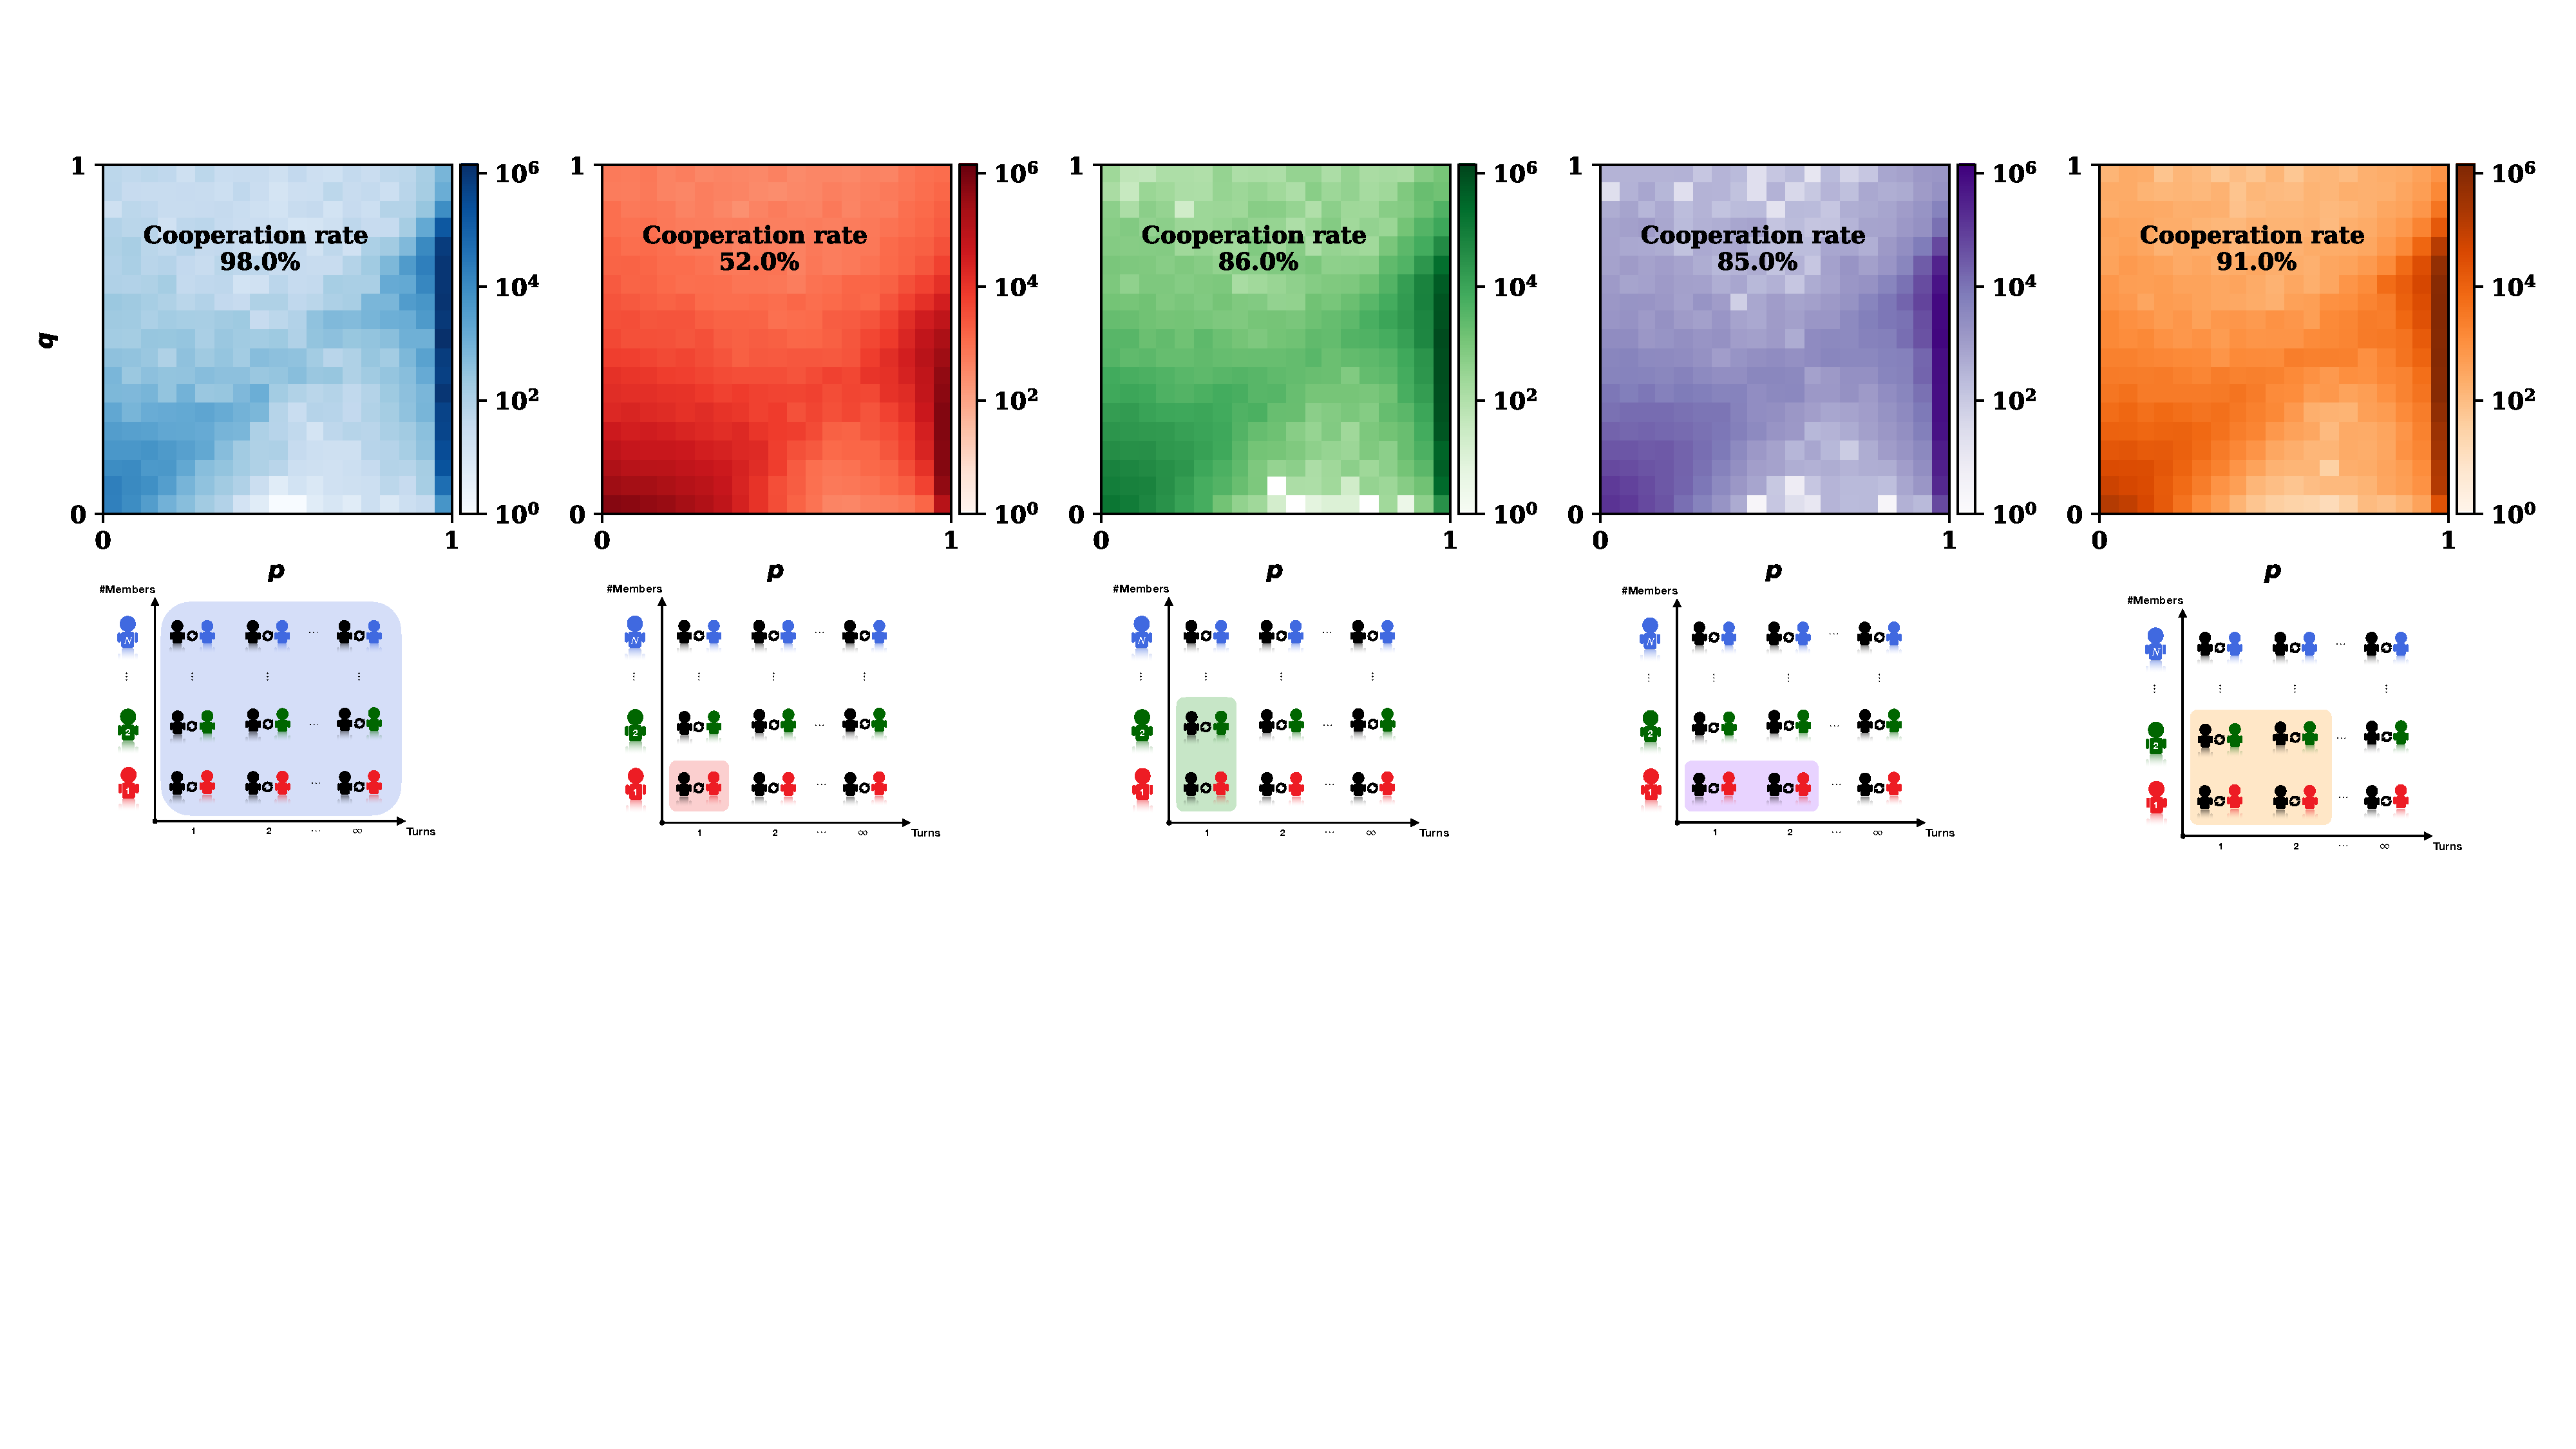
\includegraphics[width=\textwidth]{static/more_memory_heatmaps_donation_game_with_illustrations.pdf}
    \caption{\textbf{Evolutionary dynamics with difference updating approach.}
    From left to right, we present result on the following updating payoffs
    cases; the expected payoffs (perfect memory), the last round payoff
    from one interaction (limited memory), the last round payoff from two
    interactions, the last two rounds payoffs from one interaction, the
    last two rounds payoffs from two interactions. We run each simulation for \(T
    = 10^7\) time steps. For each time step we recorded the current resident
    population \((y, p, q)\). Since \(\delta \rightarrow 1\) we do not report the
    players' initial cooperation probability \(y\). The graphs show how often the
    resident population chooses each combination \((p, q)\) of conditional
    cooperation probabilities in the subsequent rounds. In both cases players
    update based on their expected payoffs.}\label{fig:expected_payoffs_results}
\end{figure}

\subsection{Expected and Last Round Updating Payoffs for Memory One Strategies}\label{section:memory_one}

So far we have assumed that individuals can adopt reactive strategies.
To demonstrate that our results hold for higher memory strategies here we
present results for the expected payoffs, and the last round payoff when members
use memory-one strategies. Memory-one strategies consider the outcome of the
previous round to decide on an action. There are four possible outcome in each
round; \((C, C), (C, D), (D, C), (D, D)\). A memory-one strategy \(s\) can be
written as a five-dimensional vector \(s=(y, p_1, p_2, p_3, p_4)\). The
parameter \(y\) is the probability that the strategy opens with a cooperation
and \(p_1\), \(p_2\), \(p_3\), \(p_4\) are the probabilities that the strategy
cooperates for each of the possible outcomes of the last round.

We perform four separate simulations where we differ the updating payoff and the
benefit of cooperation \(b\). The results for a low value of benefit are given
in Figure~\ref{fig:memory_one_low_benefit}, and for a high benefit in
Figure~\ref{fig:memory_one_high_benefit}. We verify that even when individuals
are allowed to use memory-one strategies, the cooperation rate is higher
in the perfect memory approach compared to the limited memory.

\begin{figure}[!htbp]
  \centering 
  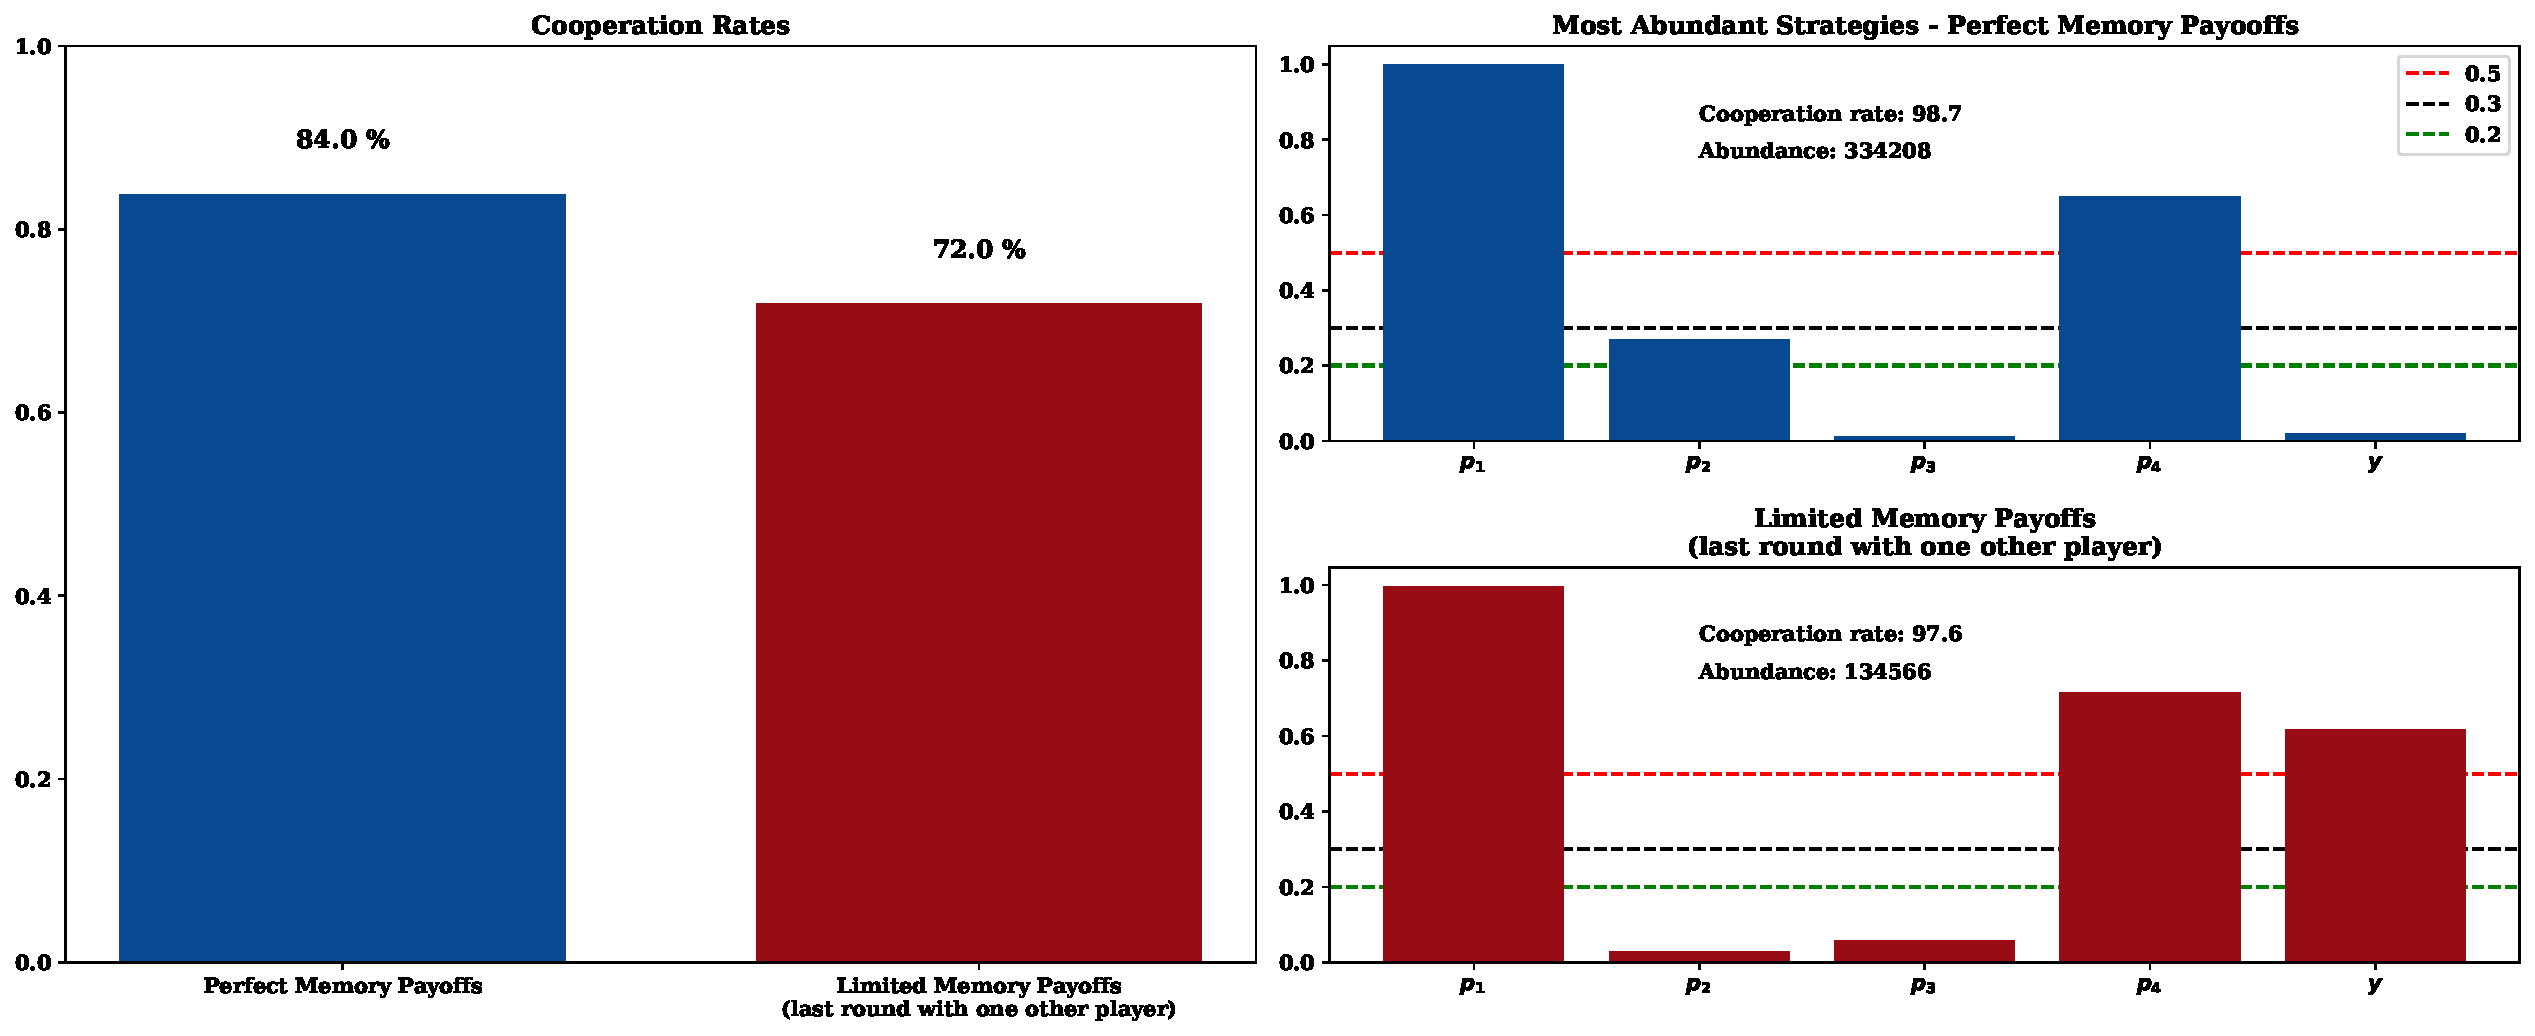
\includegraphics[width=\textwidth]{static/memory_one_results_low_benefit.pdf}
  \caption{\textbf{Evolutionary dynamics results for memory-one strategies for low benefit.}
  We perform two independent simulations. In one simulation individuals use
  expected payoffs and in the other the last round one interacts when they
  update their strategies. We run each simulation for \(T = 10^8\) time steps.
  For each time step, we have recorded the current resident population, who is
  now of the form  \((y, p_1, p_2, p_3, p_4)\) In the left panel we report the
  cooperation rates for each simulation. It can be shown than even for
  memory-one strategies expected payoffs result in a more cooperative
  population. The right panel reports the most abundant strategy of each
  simulation. Abundance is the number of mutants a strategy can repel before
  being invaded. The most abundant strategies have some similarities,
  namely, \(p_1 \approx 1\), \(p_3 \approx 0\) and \(p_4 > \frac{1}{2}\). There are also differences, in the latter
  case a strategy is more likely to open with cooperation and their tolerance to
  a \((C, D)\) outcome is almost zero. A difference between the strategies is their
  abundance. In the expected payoffs case a strategy can repel a way greater
  number of mutants. In the case of last round payoffs strategies become less
  robust. Parameters: \(N =100, c=1, b=3, \beta=1\).}\label{fig:memory_one_low_benefit}
\end{figure}


\begin{figure}[!htbp]
  \centering 
  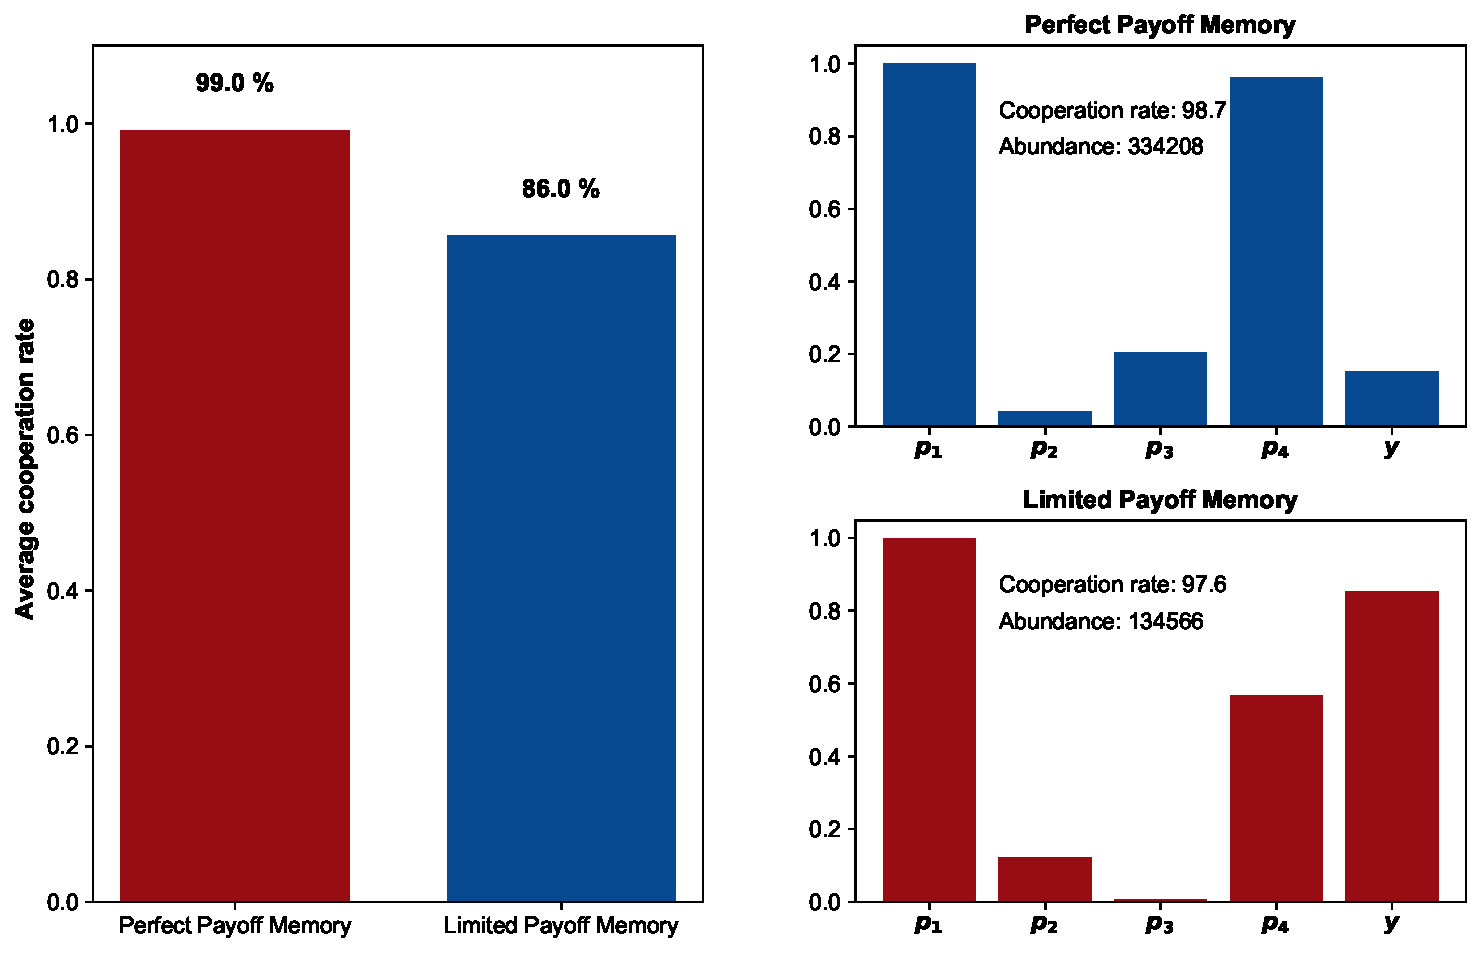
\includegraphics[width=\textwidth]{static/memory_one_results_high_benefit.pdf}
  \caption{\textbf{Evolutionary dynamics results for memory-one strategies for high benefit.}
  We perform two independent simulations. In the case of high benefit expected
  payoffs again result in a more cooperative population. The right panel reports
  the most abundant strategy of each simulation. Abundance is the number of
  mutants a strategy can repel before being invaded. For the expected payoffs he
  most abundant is that of win-stay lose-shift. However in the later case the
  most abundant strategy is a strategy with no tolerance to one defection, and
  it cooperates with a probability 0.5 after a mutual defection.  In the expected
  payoffs case strategies are more robust.  Parameters: \(N =100, c=1, b=10,
  \beta=1\).}\label{fig:memory_one_high_benefit}
\end{figure}


\subsection{Expected and Last Round Updating Payoffs for High Mutation ($\mu \neq 0$)}\label{section:mutation}

In this section we evaluate the main result of this work for \(\mu \neq 0\).
Namely, we explore the evolved population when individuals use perfect and
limited updating payoff memory for different values of \(\mu\). We perform five
independent runs of the pairwise process described in
Section~\ref{section:model}, and at each time step we record the
average player \(\bar{s}=(\bar{y}, \bar{p}, \bar{q})\). The average cooperation
of the resident population for different values of mutation are shown in
Figure~\ref{fig:mutation}. The cooperation rate in the case of perfect
memory is always higher compared to the limited memory regardless of the
mutation value. For mutation value of 1 the processes become random and
this results to a cooperation rate of \(\frac{1}{2}\) in both simulations.

\begin{figure}[!htbp]
  \centering 
  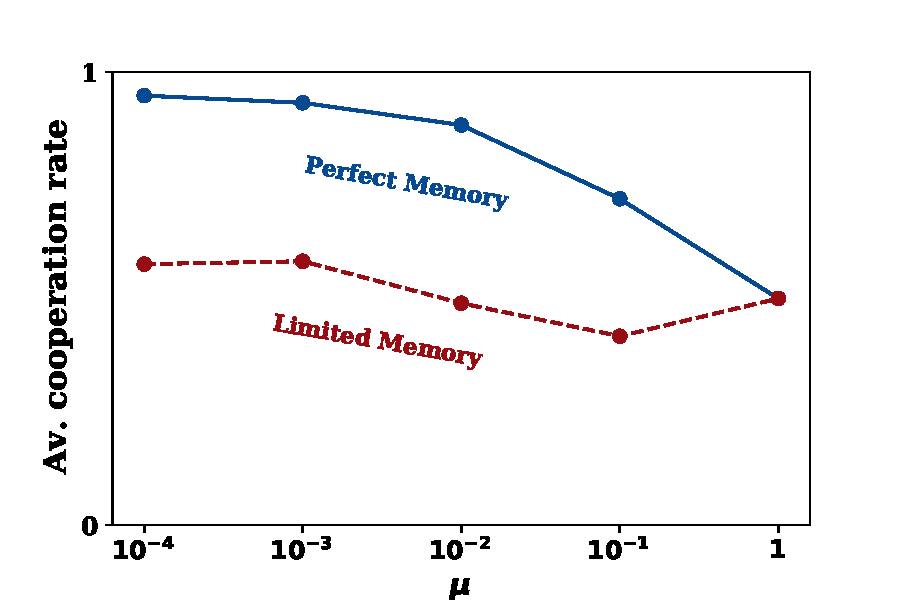
\includegraphics[width=.5\textwidth]{static/mutation_perfect_and_limited_memory_donation_game.pdf}
  \caption{\textbf{Evolutionary dynamics results for perfect and limited memory
  for different mutation values.}
  We perform five independent simulations. Simulations are run
  for $T\!=\!4\times 10^7$ time steps for each parameter. In each time step
  we introduce a new mutant with a probability \(\mu\), and we then select
  two random players to serve as the role model and the learner. The learner
  adopts the strategy of the role model with a probability \(\rho(\pi_{L}, \pi_{RM})\) where the
  updating payoffs depend on the method. In the case of perfect memory
  the expected payoffs are used and in the case of limited memory the
  last round payoff against one opponent. We plot the average cooperation rate
  within the resident population for each value of \(\mu\). For \(\mu=1\)
  the process becomes random and so the cooperation rates are 0.5. For the rest
  of the mutation values the perfect memory payoffs once again overestimate the
  evolved cooperation, confirming the results of low mutation. Parameters: \(N
  =100, c=1, b=10, \beta=1\).}\label{fig:mutation}
\end{figure}



%%%%%%%%%%%%
%% REFERENCES %%
%%%%%%%%%%%%

\clearpage
\newpage

{
{\setlength{\bibsep}{0\baselineskip}
\bibliographystyle{naturemag}
\bibliography{bibliography.bib}
}

\christian{Adjust symbols in main text -- for role model, strategy, etc}
\end{document}